% !iTeXMac(input): POH.tex
\chapter{AIRPLANE \& SYSTEMS DESCRIPTIONS} \vspace{\minitocspacebefore} \minitoc

%\minilof
\cleardoublepage

%\startcontents[chapters]
%\titleformat{\chapter}[display] {...}{...}{...} % Your definitions come here [\vspace*{4pc}% 
%\startcontents[chapters] % from titletoc 
%\printcontents{l}{1}{\setcounter{tocdepth}{2}}] % from titletoc
%% following five commands to control the placement of figures on the pages
%% these values are changed for the Performance Section to allow room 
%% for two graphs on one page, with no text outside the figure.
\renewcommand{\textfraction}{0.1} 
\renewcommand{\topfraction}{.9} 
\renewcommand{\bottomfraction}{.9} 
\renewcommand{\floatpagefraction}{0.35} \setcounter{totalnumber}{5} 

\section{AIRFRAME}

The airframe is aluminum alloy construction except for steel components comprising: engine mount, landing gear, landing gear mounts, elevator control horns and other miscellaneous items. The tips of the wings and tail surfaces as well as cowling, landing gear fairings, empennage fairings and canopy skirt are fabricated from fibreglass. The aircraft is conventionally configured with a 13.5\% thick NACA 23000 series non-laminar-flow aerofoil.

\section{COCKPIT LAYOUT}

%\textcolor{red}{Finish adding legends for instrument panel diagram.}
The flight instruments are in a ``Standard-T'' arrangement, very slightly right of centre on the main instrument panel. The engine instruments and fuel gauges are to the right side of the flight instruments, and the avionics are located to the left of the flight instruments (Figure \ref{inst-panel}). Switches that are normally only used on the ground are on a switch console on the right cockpit wall below the instrument panel (Figure \ref{right-console}). Switches that are normally used in flight are on the sub-panel to the left of the main instrument panel (Figure \ref{left-sub-panel}).

The throttle, propeller and mixture controls are in a throttle quadrant mounted on the left cockpit wall below the instrument panel. The fuel selector is on a horizontal shelf on the lower, left side of the cockpit ahead of the pilot's seat.

Engine alternate air and oil cooler door controls are mounted on the side of the left landing gear box structure, below and ahead of the instrument panel. The cockpit heat controls are mounted on the aft wall of the forward baggage compartment, below and ahead of the instrument panel to the right of the pilot's right calf. 

The parking brake control is mounted on the centre of the forward baggage compartment aft bulkhead, below and ahead of the instrument panel.

The front stick grip contains controls for pitch and roll trim, trim and autopilot cut-out, boost pump ON-OFF toggle, radio transmit, and starter engage (Figure \ref{stick-grip}).

The auxiliary power outlet is located on the lower aft face of the right landing gear box structure.

The rear seat has a throttle mounted on the left side wall, and a pitch trim switch just ahead of the throttle. There is a radio transmit push-button near the top of the bulkhead on the right side of the rear cockpit. \clearpage \vspace*{\fill} 
\begin{center}
	
	%    This page intentionally left blank.
	\Large THIS PAGE INTENTIONALLY LEFT BLANK. 
\end{center}
\vspace{\fill} \thispagestyle{empty} 
\newpage 
\begin{sidewaysfigure}
	
	\begin{overpic}
		[scale=1]{../Diagrams/Panel7} \huge
		
		% The following commands work with the pspicture package
		% \put(24,37){\ding{172}} % #1 dingbat
		% \put(25.5,36.8){\Vector(.5,-7.8)}
		% \put(20,36){\ding{173}} % #2 dingbat
		% \put(22,35.9){\Vector(1.6,-6.9)}
		% \put(15,34){\ding{174}} % #3 dingbat
		% \put(17.3,34.3){\Vector(8,-8.5)}
		% \put(3,23){\ding{175}} % #4 dingbat
		% \put(5.5,23.7){\Vector(16.5,.8)}
		% \put(10.5,30){\ding{176}} % #5 dingbat
		% \put(13,30.7){\Vector(6.5,-4)}
		% \put(15,-5){\ding{177}} % #6 dingbat
		% \put(16.6,-2.3){\Vector(1.3,3.7)}
		% \put(20.1,-5){\ding{178}} % #7 dingbat
		% \put(21.3,-2.3){\Vector(0,3.7)}
		% \put(25.1,-5){\ding{179}} % #8 dingbat
		% \put(25.9,-2.3){\Vector(-1.3,3.7)}
		% \put(94,22){\ding{180}} % #9 dingbat
		% \put(94.2,22.1){\Vector(-2,-2.9)}
		% \put(95,-5){\ding{181}} % #10 dingbat
		% \put(95.8,-2.3){\Vector(-.6,3.7)}
		% \put(96.6,-2.3){\Vector(.5,3.7)}
		% The following commands work with the pict2e package
		\put(24,37){\ding{172}} 
		
		% #1 dingbat
		\put(25.5,36.8){\vector(5,-78){0.5}} \put(20,36){\ding{173}} 
		
		% #2 dingbat
		\put(22,35.9){\vector(16,-69){1.6}} \put(15,34){\ding{174}} 
		
		% #3 dingbat
		\put(17.3,34.3){\vector(80,-85){8}} \put(3,23){\ding{175}} 
		
		% #4 dingbat
		\put(5.5,23.7){\vector(165,8){16.5}} \put(10.5,30){\ding{176}} 
		
		% #5 dingbat
		\put(13,30.7){\vector(65,-40){6.5}} \put(15,-5){\ding{177}} 
		
		% #6 dingbat
		\put(16.6,-2.3){\vector(13,37){1.3}} \put(20.1,-5){\ding{178}} 
		
		% #7 dingbat
		\put(21.3,-2.3){\vector(0,1){3.7}} \put(25.1,-5){\ding{179}} 
		
		% #8 dingbat
		\put(25.9,-2.3){\vector(-13,37){1.3}} \put(94,22){\ding{180}} 
		
		% #9 dingbat
		\put(94.2,22.1){\vector(-20,-29){2}} \put(95,-5){\ding{181}} 
		
		% #10 dingbat
		\put(95.8,-2.3){\vector(-6,37){0.6}} \put(96.6,-2.3){\vector(5,37){0.5}} 
	\end{overpic}
	\vspace{.5in}
		\begin{multicols}
		{2} 
		\begin{enumerate*}
			\item \textbf{MSTR WARN} --- Flashes when the EIS 4000 Engine Monitor detects an exceedence. 
			\item \textbf{LOW OIL PRESSURE} --- Lights when the oil pressure is less than 15 psi. 
			\item \textbf{STRTR ENGAGED} --- Lights when the starter is engaged. 
			\item \textbf{BOOST PUMP} --- Lights when electrical power is supplied to the boost pump. 
			\item \textbf{ANNUN. BRT/DIM} --- Controls the annunciator and pitch and roll trim indicator intensity. \\
			Note: The MSTR WARN annunciator is not dimmable. 
			\item \textbf{INST PANEL} --- Dims panel floodlight and Microair 760 COM back-lighting. 
			\item \textbf{AVIONICS} --- Dims Garmin GNS 430W and transponder displays. 
			\item \textbf{CDI + ENG INST} --- Dims CDI, Narco 122D and Engine instruments. 
			\item \textbf{ELT REMOTE CONTROL} 
			\item \textbf{HEADSET JACKS} 
		\end{enumerate*}
	\end{multicols}
	\vspace{.5in} \caption{Instrument Panel} \label{inst-panel} 
\end{sidewaysfigure}
\clearpage
\begin{sidewaysfigure}
	\begin{minipage}{3in}
		
		\begin{overpic}
			[scale=.6, bb = 100 78 476 708]{../Diagrams/LH_Panel} \Huge \put(44,80){\ding{172}} 
			
			% #1 dingbat
			\put(41.3,67.1){\ding{173}} 
			
			% #2 dingbat
			\put(31.4,52.2){\ding{174}} 
			
			% #3 dingbat
			\put(29.4,23.7){\ding{175}} 
			
			% #4 dingbat
			\put(40.3,23.7){\ding{176}} 
			
			% #5 dingbat
			\put(51.2,23.7){\ding{177}} 
			
			% #6 dingbat
			\put(21.2,7.1){\ding{178}} 
			
			% #7 dingbat
			\put(29.7,7.1){\ding{179}} 
			
			% #8 dingbat
			\put(40.3,7.1){\ding{180}} 
			
			% #9 dingbat
			\put(51.2,7.1){\ding{181}} 
			
			% #10 dingbat
		\end{overpic}

	\end{minipage}
	\hfill 
	\begin{minipage}{5.6in} 
		\begin{enumerate}
			\item \textbf{FLUX VALVE} --- Selects the EFIS Flux Valve OFF if required due to electromagnetic interference with COM reception. 
			\item \textbf{PITCH TRIM INDICATOR} --- Displays Pitch Trim position. Nose Up trim is to the top of the display, Nose Down trim is to the bottom. 
			\item \textbf{ROLL TRIM INDICATOR} --- Displays roll trim position. 
			\item \textbf{NAV/STR} --- Controls Navigation and Strobe Lights. Lower position is Navigation and Strobe Lights OFF. Middle position is Navigation Lights ON, and Strobe Lights OFF. Upper position is Navigation Lights and Strobe Lights ON. 
			\item \textbf{TAXI LT} --- Controls Taxi Light in left outboard wing. 
			\item \textbf{LDG LT} --- Controls Landing Light in right outboard wing. \\
			\\
			The Taxi and Landing Lights flash alternately if both switches are placed in the middle, "FLASH", position. 
			\item \textbf{IGNITION --- MAG} --- Controls the single magneto. 
			\item \textbf{IGNITION --- ELEC} --- Controls the Electronic Ignition which is installed in place of the right magneto. 
			\item \textbf{STARTER} --- Guarded switch enables the Start switch on the front control stick grip, and provides an alternate starter switch. The lower position disables the stick grip starter switch. If the guard is lifted, and the switch placed in the middle position, the stick grip starter switch is enabled. The momentary upper position engages the starter. 
			\item \textbf{FLAPS} --- Momentary switch causes the flaps to move up or down while it is held. The flap actuator will free-wheel once the flaps reach full travel up or down. 
		\end{enumerate}
	\end{minipage}
\vspace{.5in} \caption{Instrument Panel --- Left Side} \label{left-sub-panel} 
\end{sidewaysfigure}
\FloatBarrier

\begin{wrapfigure}
	[26]{r}{150pt}
	\begin{overpic}
		[scale=0.5]{../Diagrams/RH-Console} \Large \put(5,91.5){1} \put(5,83.6){2} \put(5,75.7){3} \put(5,67.8){4} \put(5,59.9){5} \put(5,52){6} \put(5,44){7} \put(5,36.1){8} \put(5,28.2){9} \put(3.4,20.3){10} \put(3.4,12.4){11} \put(3.4,4.5){12}
	\end{overpic}
	\caption{Switch Console} \label{right-console} 
\end{wrapfigure}

\textbf{Right Console} --- The following switches are on the right console, which is located on the right wall of the cockpit, below the instrument panel:

\begin{enumerate}
	\item \textbf{BATT/ALT} --- Battery Master and Main Alternator switch. Left position is both OFF, middle position is Battery Master ON, and Main Alternator OFF, and right position is both ON. 
	\item \textbf{STBY ALT} --- Standby Alternator switch. 
	\item \textbf{ESS BUS FEED} --- NORM: Essential Bus is fed from Main Bus, via a diode. EMER: Essential Bus is fed directly from Battery. 
	\item \textbf{ENG INST} --- EIS 4000 Engine Monitor power switch. 
	\item \textbf{EFIS BU} --- Backup source of power for the EFIS, from the Battery Bus. 
	\item \textbf{TURN COORD} --- Turn Coordinator power switch, from the Battery Bus. 
	\item \textbf{PITOT HEAT} --- Pitot Heat power switch. 
	\item \textbf{DFRST FAN} --- Defrost Fan power switch. 
	\item \textbf{TRIM} --- Pitch and Roll Trim power. Also selects which pitch trim switches are enabled. 
	\item \textbf{WING LVLR} --- Autopilot power switch. Controls power to the Autopilot control head and servo. 
	\item \textbf{ALT} --- Main Alternator Field Circuit Breaker. This CB will pop if the Over-voltage Protection System detects an over-voltage, removing power from the alternator field, which shuts down the alternator. 
	\item \textbf{STBY ALT} --- Standby Alternator Relay CB. This CB will pop if the Over-voltage Protection System detects an over-voltage caused by the Standby Alternator. 
\end{enumerate}

\FloatBarrier

\clearpage 
\section{STICK GRIP SWITCHES}
\begin{figure}
	[h!]
	
	\begin{minipage}{3in}
	  The front seat has an Infinity Aerospace stick grip with switches that control various aircraft systems.
		\begin{enumerate}
			\item \textbf{Trim and Autopilot Disconnect} --- Red. The power to the elevator and aileron trim servos is removed when this momentary switch is depressed. The power will be restored when the switch is released.  A press and release within 5 seconds will disconnect the autopilot.  Holding the switch depressed for longer than 5 seconds will activate the autopilot Pilot Command Steering mode.
			
			\item \textbf{Elevator and Aileron Trim} --- Controls elevator and roll trim.
			
			\item \textbf{Boost Pump} --- Blue. The ON or OFF state of the boost pump power is toggled when this switch is pressed and released. The pump ON/OFF status is indicated by the "Boost Pump" light on the instrument panel which illuminates when the boost pump is powered.
			
			\item \textbf{Trigger} --- Not used. This Push ON, Push OFF switch may eventually be used for smoke system control. 
			
			\item \textbf{PTT} --- Black. Push to Talk.
			
			\item \textbf{Starter} --- Green. Engages the starter, if the Start Enable switch on the Instrument Panel is in the Enable position. 
		\end{enumerate}
	\end{minipage}
	%\qquad
	\quad 
	\begin{minipage}{2.85in}
		
		\begin{tabular}{cc} 
			\begin{overpic}[scale=.2]{../Diagrams/stick-grip1} \Large \put(-1,95){\ding{172}} 
				
				% #1 dingbat
				%  \put(3,94){\Vector(6,-12)}
				\put(3,94){\vector(1,-2){3.5}} \put(14.25,99.25){\ding{173}} 
				
				% #2 dingbat
				%  \put(19,99){\Vector(15,-13)}
				\put(19,99){\vector(6,-5){12}} \put(55,99){\ding{174}} 
				
				% #3 dingbat
				%  \put(56,98){\Vector(-3,-7)}
				\put(56,98){\vector(-1,-2){3}} \put(-1,60){\ding{176}} 
				
				% #5 dingbat
				%  \put(3,59){\Vector(4,-8)}
				\put(3,59){\vector(1,-2){4}} \normalsize 
			\end{overpic}
			&
			\begin{overpic}[scale=.17]{../Diagrams/stick-grip2} \Large \put(-6.25,43.25){\ding{175}} 
				
				% #4 dingbat
				%  \put(-2,48){\Vector(5,8)}
				\put(-2,48){\vector(2,4){4}} \put(1.5,35){\ding{177}} 
				
				% #6 dingbat
				%  \put(5,34){\Vector(7,-16)}
				\put(5,34){\vector(1,-2){7}} \normalsize 
			\end{overpic}
		\end{tabular}
		\caption{Stick Grip Switches} \label{stick-grip}
		
	\end{minipage}
\end{figure}
\FloatBarrier

\section{CANOPY}

\textbf{Canopy Latch} --- The canopy is latched by a handle and hook at the left front side of the sliding canopy frame. The handle may rotate and the hook may release if the handle is hit in flight, but the air loads push the canopy forward, so there is no risk of it departing the aircraft.

\textbf{Canopy Jettison} --- The front canopy bow is attached to the rollers by ``Pip'' pins that can be pulled by the pilot, thus allowing the front of the canopy to be released from the rails. The canopy jettison procedure is:
\begin{enumerate*}
	\item Canopy ``Pip'' pins --- PULL 
	\item Canopy Latch --- UNLATCH 
	\item Canopy --- PULL AFT and PUSH UP 
	\item Head --- DUCK to prevent getting hit by canopy as it departs the aircraft 
\end{enumerate*}
\begin{Note}
	[WARNING] The canopy may hit the tail as it departs the aircraft, so the canopy should only be jettisoned if it is intended to abandon the aircraft. 
\end{Note}

\section{ENGINE AND PROPELLER}

The aircraft is powered by a Lycoming I0-360-A1B6 four cylinder, direct drive, horizontally opposed engine rated at 200 HP at 2700 rpm. The engine is fitted with a 60 amp 14 volt main alternator, an 8 amp standby alternator, shielded magneto ignition, Lightspeed Engineering electronic ignition, fuel pump, fuel injection, and an alternate air induction system.

The exhaust system is all stainless steel with a crossover configuration and no mufflers. Two heat muffs provide cabin heat.

The engine drives a 72.05\char`\"{} (183 cm) diameter MT three-blade constant speed propeller.  The propeller blade roots have counterweights that force them towards coarse pitch if propeller governor oil pressure is lost.  The propeller blades are of composite construction, with a wooden core covered by epoxy fibreglass.  The outer portion of the blade leading edges is protected by a stainless steel erosion strip that is bonded in place.  The inner portion of the blade leading edge is protected by a self-adhesive strip.

\section{ENGINE MONITOR} 
\begin{wrapfigure}[15]{R}{0pt}
	
	
\includegraphics{../Diagrams/eis1} \caption{EIS 4000 Engine Monitor} 
\end{wrapfigure}

The Grand Rapids EIS 4000 Engine Information System (EIS) is located on the lower right side of the main instrument panel, and is powered from the Essential Bus, through the ``ENG INST'' switch on the right switch panel. The EIS 4000 displays the following engine parametres:
\begin{itemize*}
	\item RPM 
	\item Manifold Pressure (in HG) 
	\item Oil Temperature (\textdegree F) 
	\item Oil Pressure (\textdegree F) 
	\item Cylinder Head Temperature --- all cylinders (\textdegree F) 
	\item Exhaust Gas Temperatures --- all cylinders (\textdegree F) 
	\item Fuel Flow (USG/hr) 
	\item Fuel Remaining (USG) 
	\item Fuel Pressure ($\mathrm{lb/in^{2}}$) 
	\item Essential Bus Voltage (v)
	\item Outside Air Temperature (\textdegree F) from sensor mounted in NACA scoop under right wing. 
\end{itemize*}

\subsection*{Alarms}

%\textbf{Alarms} --- Each parametre that the EIS monitors can have upper and lower limits assigned, and the EIS will annunciate an alarm condition if these limits are breached.
Each parametre that the EIS monitors can have upper and lower limits assigned, and the EIS will annunciate an alarm condition if these limits are breached. The ``MSTR WARN'' red light will flash (upper left side of instrument panel), and the EIS display will change pages to show the affected parametre flashing above its label. If the parametre returns within the allowable range, the ``MSTR WARN'' light will extinguish, and the display will automatically return to the previously displayed page. The alarm can be reset by pressing the ``Next/Ack'' on the EIS. The ``MSTR WARN'' light will stop flashing, but will remain illuminated as long as any parametre remains outside the allowable range. The display will change to the previously displayed page.

\subsection*{Display Formats}

%\textbf{Displays} --- There are 14 different pages of data that may be displayed.  
There are 14 different pages of data that may be displayed. Pressing the ``Next/Ack'' button cycles to the next page. Pressing the ``Previous'' button cycles to the previous page. Double-pushing the ``Display'' button changes to the default page. The two user-configurable pages don't have labels identifying which parametre each block of numbers represents. Pressing and holding the ``Display'' button from a user-configurable page replaces the digits with the data labels, allowing the data blocks to be identified.
\clearpage 
The pages, in sequence, are:

% The following lengths define extra space to be left between the hlines and the text in the page format table.
\newlength{\tabletopspace} 
\setlength{\tabletopspace}{.5ex} 
\newlength{\tablebottomspace}
\setlength{\tablebottomspace}{.5ex}

% The following lengths control the table width
\newlength{\eistableleftcol} 
\setlength{\eistableleftcol}{1.2in}
% \settowidth{\eistableleftcol}{3:38 38.2 10.5 Endur Fuel Flow}
\newlength{\eistablerightcol} 
\setlength{\eistablerightcol}{\textwidth-\eistableleftcol-0.35in}
\begin{longtable}
	{|l|l|} \hline \multicolumn{1}{|c|}{\bfseries{EIS Page Layout}}&\multicolumn{1}{c|}{\bfseries{Remarks}}\\
	\hline\hline
\endfirsthead \multicolumn{2}{l}{\emph{Continued from previous page}}\\
\hline \multicolumn{1}{|c|}{\bfseries{EIS Page Layout}}&\multicolumn{1}{c|}{\bfseries{Remarks}}\\
\hline\hline 
\endhead \hline \multicolumn{2}{r}{\hfill \emph{Continued on next page}}\\
\endfoot \hline 
\endlastfoot

%% Fuel
\begin{minipage}{\eistableleftcol}\ttfamily 
\begin{verbatim}3:38  38.2  10.5
Endur Fuel  Flow\end{verbatim}
\end{minipage}&
\begin{minipage}{\eistablerightcol}
\vspace{\tabletopspace}
\textbf{Fuel Page }\\
\textbf{Top row} --- Endurance to dry tanks (H:M), Fuel Quantity (USG) and Fuel Flow (USG/hr).\\
\textbf{Bottom row} --- Data labels.

The fuel quantity is a detotalizer, based on the pilot-entered fuel quantity, less the integrated fuel flow.

% \centering \textbf{WARNING}
% 
% The fuel flow is not yet calibrated, so the detotalizer is not accurate.  \\
% The fuel gauges are the primary source of fuel quantity information.
\vspace{\tablebottomspace}
\end{minipage}\\
\hline

%%User page 1
\begin{minipage}{\eistableleftcol}
  \ttfamily {2410/23.0\ \ \ \ 400\\
200/70 10.5 1335} 
\end{minipage}
& 
\begin{minipage}{\eistablerightcol} 
  \vspace{
\tabletopspace} \textbf{User-configurable Page 1 --- Default Page}\\
\textbf{Top row} --- RPM/MP Highest CHT\\
\textbf{Bottom row} --- Oil Temperature/Oil Pressure, Fuel Flow (USG/hr), Highest EGT\\\\
Press and hold the ``Display'' button to replace the digits with data labels.\\
Double-push the ``Display'' button to switch to this page from any other page. \vspace{
\tablebottomspace} 
\end{minipage}
\\
\hline

%%User page 2
\begin{minipage}{\eistableleftcol}\ttfamily {36.8\ \ 10.8\ \ \ \ 29\\
-10\textdegree\ \ 13.6\ \ \ 0.0}
\end{minipage}&
\begin{minipage}{\eistablerightcol}
\vspace{\tabletopspace}
\textbf{User-configurable Page 2}\\
\textbf{Top row} --- Fuel Quantity (USG), Fuel Flow (USG/hr) and Fuel Pressure ($\mathrm{lb/in^{2}}$).\\
\textbf{Bottom row} --- OAT (\textdegree F), Essential Bus Voltage and Main Alternator Load (amps)\\\\
Press and hold the ``Display'' button to replace the digits with data labels.
\vspace{\tablebottomspace}
\end{minipage}\\
\hline

%%EGT/CHT Bar Graph Page
\begin{minipage}{\eistableleftcol}
\setlength{\unitlength}{1.31pt}
  \ttfamily {\begin{picture}(66,9)
    \linethickness{\unitlength}
    \put (0,0){\line(10,0){5}}
    \put (0,2){\line(10,0){5}}
    \put (0,4){\line(10,0){5}}
    \put (0,6){\line(10,0){5}}
    \put (6,0){\line(1,0){2}}
    \put (9,0){\line(1,0){2}}
    \put (6,2){\line(1,0){1}}
    \put (8,2){\line(1,0){3}}
    \put (6,4){\line(1,0){2}}
    \put (9,4){\line(1,0){2}}
    \put (6,6){\line(1,0){2}}
    \put (9,6){\line(1,0){2}}
    \put (12,0){\line(10,0){5}}
    \put (12,2){\line(10,0){5}}
    \put (12,4){\line(10,0){5}}
    \put (12,6){\line(10,0){5}}
    \put (18,0){\line(10,0){5}}
    \put (18,2){\line(10,0){5}}
    \put (18,4){\line(10,0){5}}
    \put (18,6){\line(10,0){5}}
    \put (24,0){\line(10,0){3}}
    \put (24,2){\line(10,0){1}}
    \put (24,4){\line(10,0){2}}
    \put (24,6){\line(10,0){4}}
    \put(40,0){2\ \ -50}
    \end{picture}
  \begin{picture}(66,9)
    \put(0,0){10.5 \ 1335 \ 2410}
    \end{picture}}
\end{minipage}&
\begin{minipage}{\eistablerightcol}
\vspace{\tabletopspace}
\textbf{EGT/CHT Bar Graph Page}\\
\textbf{Top row} --- EGT/CHT Bar Graph --- shows the EGT for each cylinder, with the CHT as a missing pixel.  
Then, the cylinder \# of the first cylinder to peak is shown, plus its change from the peak EGT. \\
\textbf{Bottom row} --- Fuel flow, EGT for first cylinder to peak and RPM.
\vspace{\tablebottomspace}
\end{minipage}\\
\hline

%%EGT Cruise Bar Graph Page
\begin{minipage}{\eistableleftcol}
\setlength{\unitlength}{1.31pt}
  \ttfamily {\begin{picture}(66,9)
    \linethickness{\unitlength}
    \put (16,6){\line(10,0){1}}
    \put (18,6){\line(10,0){5}}
    \put (24,0){\line(10,0){3}}
    \put (24,2){\line(10,0){1}}
    \put (24,4){\line(10,0){2}}
    \put(40,0){2\ \ -50}
    \end{picture}
  \begin{picture}(66,9)
    \put(0,0){10.5 \ 1335 \ 2410}
    \end{picture}}
\end{minipage}&
\begin{minipage}{\eistablerightcol}
\vspace{\tabletopspace}
\textbf{EGT Cruise Bar Graph Page}\\
\textbf{Top row} --- EGT Cruise Bar Graph --- shows how the EGT for each cylinder has changed from the saved lean point. 
Each pixel is 10\textdegree F.  Bars growing left of centre show decrease in EGT, to the right is an increase in EGT.  
Then, the cylinder \# of the first cylinder to peak is shown, then its EGT vs the peak EGT.\\
\textbf{Bottom row} --- Fuel flow, EGT for first cylinder to peak and RPM.
\vspace{\tablebottomspace}
\end{minipage}\\
\hline

%% EGT Page
\begin{minipage}{\eistableleftcol}\ttfamily 
  \begin{verbatim}1335 1325      E
1330 1325      G\end{verbatim}
\end{minipage}&
\begin{minipage}{\eistablerightcol}
\vspace{\tabletopspace}
\textbf{EGT Page }\\
\textbf{Top row} --- EGT \#2 EGT \#1\\
\textbf{Bottom row} ---  EGT \#4 EGT \#3\\\\
The EGT presentation is oriented as if the viewer was looking down on the engine.  I.e. the top row shows the EGTs for
the front two cylinders, and the bottom row shows the rear two cylinders.
\vspace{\tablebottomspace}
\end{minipage}\\
\hline

%% Digital Leaning Page
\begin{minipage}{\eistableleftcol}\ttfamily
  \begin{verbatim} -12  -25      2
 -15 1335      L
\end{verbatim}
\end{minipage}&
\begin{minipage}{\eistablerightcol}
\vspace{\tabletopspace}
\textbf{Digital Leaning Page }\\
\textbf{Top row} --- EGT \#2 EGT \#1\\
\textbf{Bottom row} ---  EGT \#4 EGT \#3\\\\
Shows the EGTs for all cylinders that have not peaked.  
Once an EGT reaches peak, and decreases by 10\textdegree F, the EGT is replaced by the amount the temperature has
decreased from the peak.  
The cylinder \# for the first cylinder to peak is shown in the top right corner of the display.  \textbf{Note that the
numbering scheme here is not the same as Lycoming's cylinder numbering scheme} --- 1 is top left (Cyl \#2), 2 is top right (Cyl \#1), 3 is bottom left (Cyl \#4) and 4 is bottom right (Cyl \#3). 
\vspace{\tablebottomspace}
\end{minipage}\\
\hline

%% Cruise Page
\begin{minipage}{\eistableleftcol}\ttfamily
\begin{verbatim} -12   15      C
  10    5      Z\end{verbatim}
\end{minipage}&
\begin{minipage}{\eistablerightcol}
\vspace{\tabletopspace}
\vspace{.25ex}
\textbf{Cruise Page }\\
\textbf{Top row} --- EGT \#2 EGT \#1\\
\textbf{Bottom row} ---  EGT \#4 EGT \#3\\\\
Shows the amount the EGTs have changed since ``SAVE LEAN PT.'' was selected.
\vspace{.25ex}
\vspace{\tablebottomspace}
\end{minipage}\\
\hline

%% CHT Page
\begin{minipage}{\eistableleftcol}\ttfamily 
\begin{verbatim} 385  400    400
 390  395    CHT\end{verbatim}
\end{minipage}&
\begin{minipage}{\eistablerightcol}
\vspace{\tabletopspace}
\textbf{CHT Page }\\
\textbf{Top row} --- CHT \#2 CHT \#1  plus highest CHT in top right corner.\\
\textbf{Bottom row} ---  CHT \#4 CHT \#3\\\\
The CHT presentation is oriented as if the viewer was looking down on the engine.  I.e. the top row shows the CHT for
the front two cylinders, and the bottom row shows the rear two cylinders. 
\vspace{\tablebottomspace}
\end{minipage}\\
\hline

%% Flight Timer Page
\begin{minipage}{\eistableleftcol}\ttfamily 
1:22:57\ \ \ \ \ 108\textdegree \\
191.5 Hour\ \ Unit
\end{minipage}&
\begin{minipage}{\eistablerightcol}
\vspace{\tabletopspace}
\textbf{Timer/Temperature Page }\\
\textbf{Top row} --- Flight Timer --- runs when the RPM is above 2000 rpm.  Shows the last flight time at power up, and
the current flight time after three minutes of flight.  Hours:Minutes:Seconds.  The internal unit temperature is shown
in the top right corner.\\
\textbf{Bottom row} --- Engine Hours --- accumulates when the RPM is above 2000 rpm. 
\vspace{\tablebottomspace}
\end{minipage}\\
\hline

%% RPM, OT & OP
\begin{minipage}{\eistableleftcol}\ttfamily 
\begin{verbatim}2410  195     82
RPM   OilT  OilP\end{verbatim}
\end{minipage}&
\begin{minipage}{\eistablerightcol}
\vspace{\tabletopspace}
\textbf{RPM, Oil Temperature and Oil Pressure Page }\\
\textbf{Top row} --- RPM, Oil Temperature (\textdegree F) and Oil Pressure ($\mathrm{lb/in^{2}}$).\\
\textbf{Bottom row} --- Data labels.
\vspace{\tablebottomspace}
\end{minipage}\\
\hline

%% MP & Fuel Pressure
\begin{minipage}{\eistableleftcol}\ttfamily 
\begin{verbatim}24.6    0   32.0
MP           FP\end{verbatim}
\end{minipage}&
\begin{minipage}{\eistablerightcol}
\vspace{\tabletopspace}
\textbf{Manifold and Fuel Pressure Page }\\
\textbf{Top row} --- Manifold Pressure (in HG), Aux 2 input (not used) and Fuel Pressure ($\mathrm{lb/in^{2}}$).\\
\textbf{Bottom row} --- Data labels.
\vspace{\tablebottomspace}
\end{minipage}\\
\hline

%% OAT & Voltage
\begin{minipage}{\eistableleftcol}\ttfamily 
\begin{verbatim} 24   13.4   0.0
OAT   Volt  Load\end{verbatim}
\end{minipage}&
\begin{minipage}{\eistablerightcol}
\vspace{\tabletopspace}
\textbf{OAT, Voltage and Alternator Load Page }\\
\textbf{Top row} --- OAT (\textdegree F), Essential Bus Voltage and Main Alternator Load (amps).\\
\textbf{Bottom row} --- Data labels.
\vspace{\tablebottomspace}
\end{minipage}\\
\hline

%% CRate & EGT Span
\begin{minipage}{\eistableleftcol}\ttfamily 
\begin{verbatim} 13    45    -28
CRate EGTSp Carb\end{verbatim}
\end{minipage}&
\begin{minipage}{\eistablerightcol}
\vspace{\tabletopspace}
\textbf{CHT Rate of Cooling and EGT Span Page }\\
\textbf{Top row} --- Cylinder Head rate of cooling (\textdegree F/mn) and EGT Span between hottest and coolest EGT
(\textdegree F).\\
\textbf{Bottom row} --- Data labels.

\centering NOTE\\
Ignore the data labelled ``Carb''.  It is not operative.
\vspace{\tablebottomspace}
\end{minipage}\\
\hline

\end{longtable}

\begin{Note}
The tachometer signal is from the Magneto. The RPM will read "0" if the IGNITION --- MAG switch is selected OFF. 
\end{Note}

\subsection*{Setting Alarm Limits}
The upper and lower alarm limits, and other user-modifiable data, may be edited via the ``Set Limits'' function, accessed by pressing and holding the ``Next/Ack'' and `` Previous'' buttons. This brings up a long series of pages where individual parametres may be adjusted, using ``soft'' labels above each of the EIS keys. After the desired parametres are modified, normal operation is resumed by pressing and holding the ``Display'' button (which will have a soft label of ``Next'') to quickly scroll through the pages until the final page is reached, or by cycling the EIS power OFF then ON, via the ENG INST switch on the right console.

\subsection*{Normal Operation}

After power-up, the EIS will alarm for any parametres that are outside the allowable limits, such as oil pressure, fuel pressure, etc. Acknowledge each alarm in turn by a momentary press of the ``Next/Ack'' button. The unit will default to the User-Configurable Page 1, which has RPM, MP, highest CHT and EGT, Oil Pressure, Oil Temperature and Fuel Flow. Pressing and holding the ``Display'' button will replace the data with the data labels, so each field may be identified. A press of the ``Next/Ack'' button will bring up User-Configurable Page 2, which has Fuel Quantity, Fuel Flow, Fuel Pressure, OAT, Voltage and Main Alternator Load. There are 14 different pages in all --- a double-push of the ``Display'' button will return to the default page.

\textbf{Fuel Detotalizer} --- Upon power-up the fuel detotalizer function will start with the fuel quantity it had at the last power-down.  Press and hold the left and right buttons to reach the fuel quantity page.  Once on the fuel quantity page, the fuel quantity may be adjusted as indicated by the ``Soft'' labels.  The fuel quantity can be quickly set to 43 USG (full tanks) by simultaneously pushing the buttons indicated by the ``Inc'' and ``Dec'' labels.  \textcolor{red}{Confirm info on setting fuel quantity.}

\textbf{Digital Leaning Page} --- The digital leaning page is a special page that is intended to be used when leaning the mixture. This page is identified by the ``L'' in the lower right corner. Initially it shows the highest EGT for each cylinder, until each cylinder's EGT peaks, in which case it shows the EGT decrease from peak. The first cylinder to peak is identified by the digit in the top right corner of the window. Note that the numbering scheme here is not the same as Lycoming's cylinder numbering scheme --- 1 is top left (Cyl \#2), 2 is top right (Cyl \#1), 3 is bottom left (Cyl \#4) and 4 is bottom right (Cyl \#3). 

The page is used as follows: 
\begin{enumerate}
\item Select the Digital Lean Page, identified by the ``L'' in the lower right corner. 
\item Select the ``Save Lean Point?'' window, by a momentary press of the centre and right buttons, and select ``RESET''. This resets the highest EGTs to the current values. 
\item Slowly lean the engine. The EGTs should all increase, and the highest EGT for each cylinder will be continually updated. 
\item As leaning continues, one cylinder will reach peak EGT. Once the EGT was decreased by 10\textdegree F below peak the display will change to now show the number of degrees that the cylinder is less than the peak EGT. The first cylinder to peak is identified by the digit in the top right corner of the window. Note that the numbering scheme here is not the same as Lycoming's cylinder numbering scheme --- 1 is top left (Cyl \#2), 2 is top right (Cyl \#1), 3 is bottom left (Cyl \#4) and 4 is bottom right (Cyl \#3).  
\item Enrichen or lean as desired so all cylinders are at the desired value lower than the peak EGT.
\end{enumerate}

\subsection*{Abnormal Operations} The EIS will flash the ``MSTR WARN'' red light if any parametre goes outside the upper or lower limits programmed via the ``Set Limits'' interface. The EIS display will automatically change to a page that displays the parametre of interest, with the value flashing.  Press the ``Next/Ack'' button to acknowledge the warning --- the EIS display will return to its previous page.  The ``MSTR WARN'' light will stop flashing, but will remain illuminated until all parametres are within the programmed ranges.  If another parametre goes outside the programmed ranges, the ``MSTR WARN'' light will flash again, and the display will change to show the parametre of interest.

\section{ENGINE CONTROLS} Engine controls consist of throttle, propeller, mixture, alternate air door and oil cooler door controls. The throttle, propeller and mixture controls are in a throttle quadrant mounted on the left side of the front cockpit. The alternate air door position is controlled by a push-pull Bowden cable connected to a knob mounted on the upper, inboard side of the left landing gear box structure, underneath and ahead of the instrument panel. The oil cooler door controls the amount of air that enters the oil cooler, to allow the oil temperature to be varied. The oil cooler door position is controlled by a push-pull Bowden cable connected to a knob mounted on the upper, inboard side of the left landing gear box structure, underneath and ahead of the instrument panel.

\section{LANDING GEAR} The landing gear is of conventional configuration with steel landing gear legs. The tail wheel is full castering --- it is normally locked and follows the rudder position, but unlocks to a castering condition if full rudder is applied.

The main gear wheels are fitted with Cleveland 199-102 wheels and disk brakes. The tail wheel is solid rubber.

\section{BRAKES} The braking system consists of toe brakes attached to the rudder pedals operating two Cleveland brake master cylinders. The left and right brake master cylinders share a common fluid reservoir installed on the top left front face of the fire wall. Care must be taken to avoid applying brake pressure when using rudder on the ground.

%Both brake pedals should have a similar feel and a firm resistance
%after \textcolor{yellow}{\_}\char`\"{} of pedal travel.
The parking brake control valve is mounted on the forward baggage compartment aft bulkhead, below and forward of the instrument panel. The valve cannot be seen with the head in the normal flying position, but it can be felt if the hand is placed below the instrument panel, and it can be seen if the head is lowered. The control lever is on the left side of the braking brake valve, and has a spring loaded catch to secure it in the OFF position. The parking brake is OFF if the control lever is rotated vertically upwards, and it is ON if the control lever is rotated vertically downwards. 
\begin{Note}
[WARNING] The parking brake valve must be checked prior to landing to ensure that it is held in the OFF position by the spring-loaded catch. If the parking brake valve is in the ON position, any applied brake cannot be released, which may lead to loss of directional control. 
\end{Note}
\begin{Note}
[WARNING] The brakes have enough brake energy capacity for a single maximum braked rejected take-off or landing from normal approach speed.  Multiple hard braking events, or a maximum braked landing from an abnormally high landing speed could overheat the brakes resulting in brake failure. 
\end{Note}

\textcolor{red}{ADD PHOTO OR DRAWING OF PARKING BRAKE VALVE LOCATION}

\section{FLIGHT CONTROLS}

%Flight control integrity is essential for safe flight. At installation
%or after maintenance it should be confirmed that ALL controls are
%connected, secured and safeties and that they all operate within the
%specified ranges smoothly and in the correct direction. Full travel
%should be confirmed prior to each flight. NO play should be permitted
%in the control hinges; sloppiness may induce flutter. Similarly trim
%tabs must be free of play. 
%
Dual controls are fitted. A pin at the base of the passenger control stick allows it to be removed without affecting the operation of the remaining controls. Elevator and ailerons are operated through a system of adjustable push rods. The rudder is operated through a cable system to the rudder pedals.
%Rudder control from the rear seat position is by pads connected to push rods that are connected to the rudder cables. 

Pitch trim is by a tab on the right elevator actuated by an electric servo. Roll trim is by a spring bungee system actuated by an electric servo. Pitch and roll trim are selected by a ``Coolie Hat'' switch on the pilot's stick grip. Pitch trim can also be selected by a spring loaded switch ahead of the rear seat throttle lever. Trim positions are shown on LCD indicators located on the upper left portion of the instrument panel. Trim system power can be selected to OFF, FRONT or FRONT + REAR by a three position switch on the right console. Trim system power will also be removed while the red TRIM + WING LEVELER cut-out switch on the pilot's stick is depressed.

Flaps are operated electrically and are controlled by a switch mounted on the left side of the instrument panel.

\section{FUEL SYSTEM} Fuel is stored in two 21.5 US gallon tanks secured to the leading edge structure with screws and plate nuts. Fuel drains are fitted to the lowest point of each tank (and of the fuel system) and should be opened prior to the first flight of the day and after each refuelling to check for sediment and water.

The left tank is fitted with an inverted fuel pickup, which is a weighted length of flexible line, with a fuel pickup at the loose end. This introduces additional failure modes for the left tank --- the fuel pickup could get hung up inside the tank, or it could become disconnected at the front end. These failures would increase the amount of unusable fuel in the left tank by several gallons.
\begin{Note}
[WARNING] Never assume that all fuel in the left tank is usable. The left tank must not be selected for takeoff or landing unless there are at least \textcolor{red}{10 USG} of fuel remaining in that tank. If it is planned to use most of the fuel on a flight, the left tank must be used to a low value while adequate fuel still remains in the right fuel tank to safely land the aircraft in case the left fuel tank feed ceases prematurely. 
\end{Note}

The fuel selector valve is located to the left of the pilot's seat on the lower console. A knob on the valve handle must be lifted to change the selection to or from the OFF position.

A fuel gascolator is located in the left wing root area. This is not the lowest point in the fuel system and is intended as a dirt trap only prior to fuel entering the fuel pumps. The gascolator should be drained prior to the first flight of the day --- the fuel selector must be selected to LEFT or RIGHT to allow fuel to flow through the gascolator so it can be drained.

An electric boost pump is fitted in case of failure of the engine-driven fuel pump and is also used during takeoff and landing. The boost pump is controlled by the green ON/OFF toggle push button on the pilot's control stick. The green boost pump lamp on the upper left instrument panel will illuminate when electrical power is supplied to the boost pump.

The fuel filter is located on the engine side of the firewall, and is in the system between the boost pump and the engine-driven fuel pump.

A fuel flow transducer is fitted between the \textcolor{red}{fuel filter and the engine-driven fuel pump}. The fuel flow information is fed to the Grand Rapids EIS 4000, which has a detotalizer function that calculates predicted fuel remaining. The fuel quantity information in the EIS 4000 must be updated whenever fuel is added to or drained from the fuel tanks.
\begin{Note}[WARNING]The displayed fuel remaining value does not take into account any possible fuel leaks, or erroneous input of starting fuel quantity. 
\end{Note}

A fuel pressure transducer is mounted between the engine-driven fuel pump and the fuel injection servo. The fuel pressure is monitored and alarmed by the Grand Rapids EIS 4000.
\begin{figure}
[hb!] 
\begin{center}
\includegraphics*[scale = 0.4]{../Diagrams/Fuel_system4}
\end{center}

%\scalebox{.4}{\input{../Diagrams/Fuel_system5}}
%\input{../Diagrams/Fuel_system5}
\caption{Fuel System} 
\end{figure}
\clearpage 

%force fuel system figure to appear, before moving on to next system
\section{ELECTRICAL SYSTEM} 
\begin{wrapfigure}
[40]{R}{0pt} 
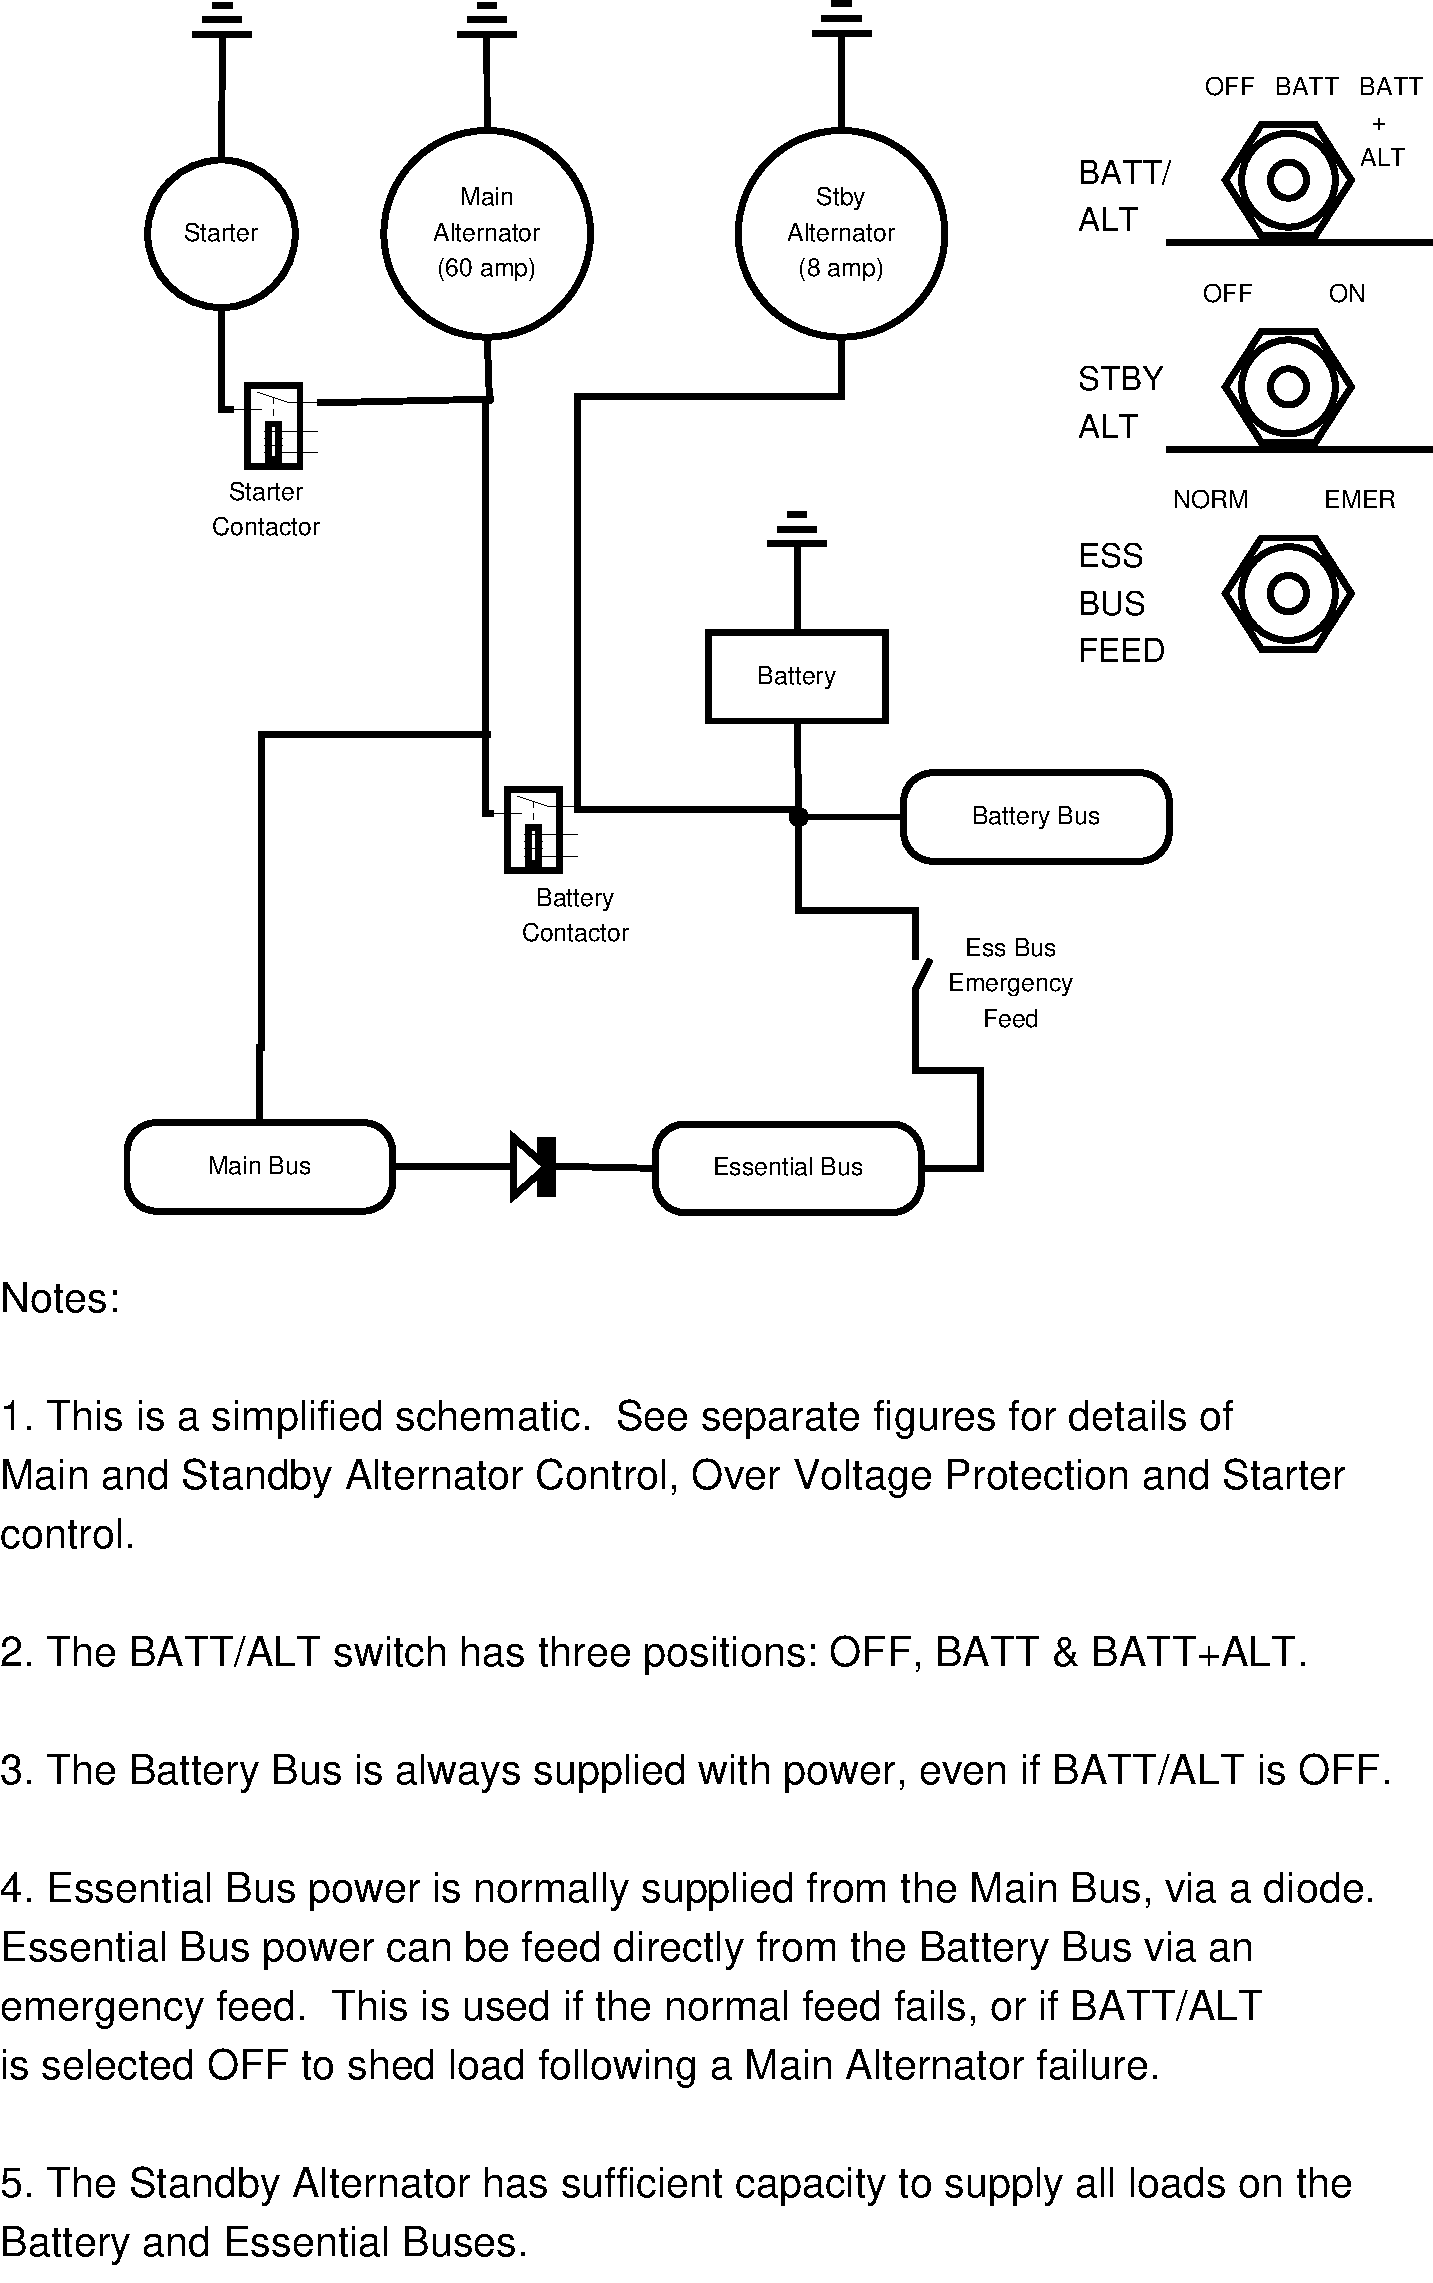
\includegraphics[clip,scale=0.4]{../Diagrams/Electrical_system_large_note} \caption{Electrical System} 
\end{wrapfigure}

The electrical system includes a 14 volt 60 amp Main Alternator, a 12 volt, 17 amp-hour battery, over voltage protection, an 8 amp Standby Alternator and a Battery Contactor. Power is distributed to Main, Essential and Battery Buses. Normally the Main Bus is powered from the Battery and Main Alternator, and the Essential Bus is powered from the Main Bus via a diode. The Battery Bus is powered all the time, regardless of the state of the Battery Contactor. The Essential Bus has a selectable alternate feed path from the Battery Bus. This alternate feed path is used if the power supplied from the Main Bus has failed, or if the Main Bus is manually shed following Main Alternator failure. An Aux Power outlet provides 10A of Battery Bus power for handheld devices. It may also be used to charge the battery.

\begin{figure}
\centering 
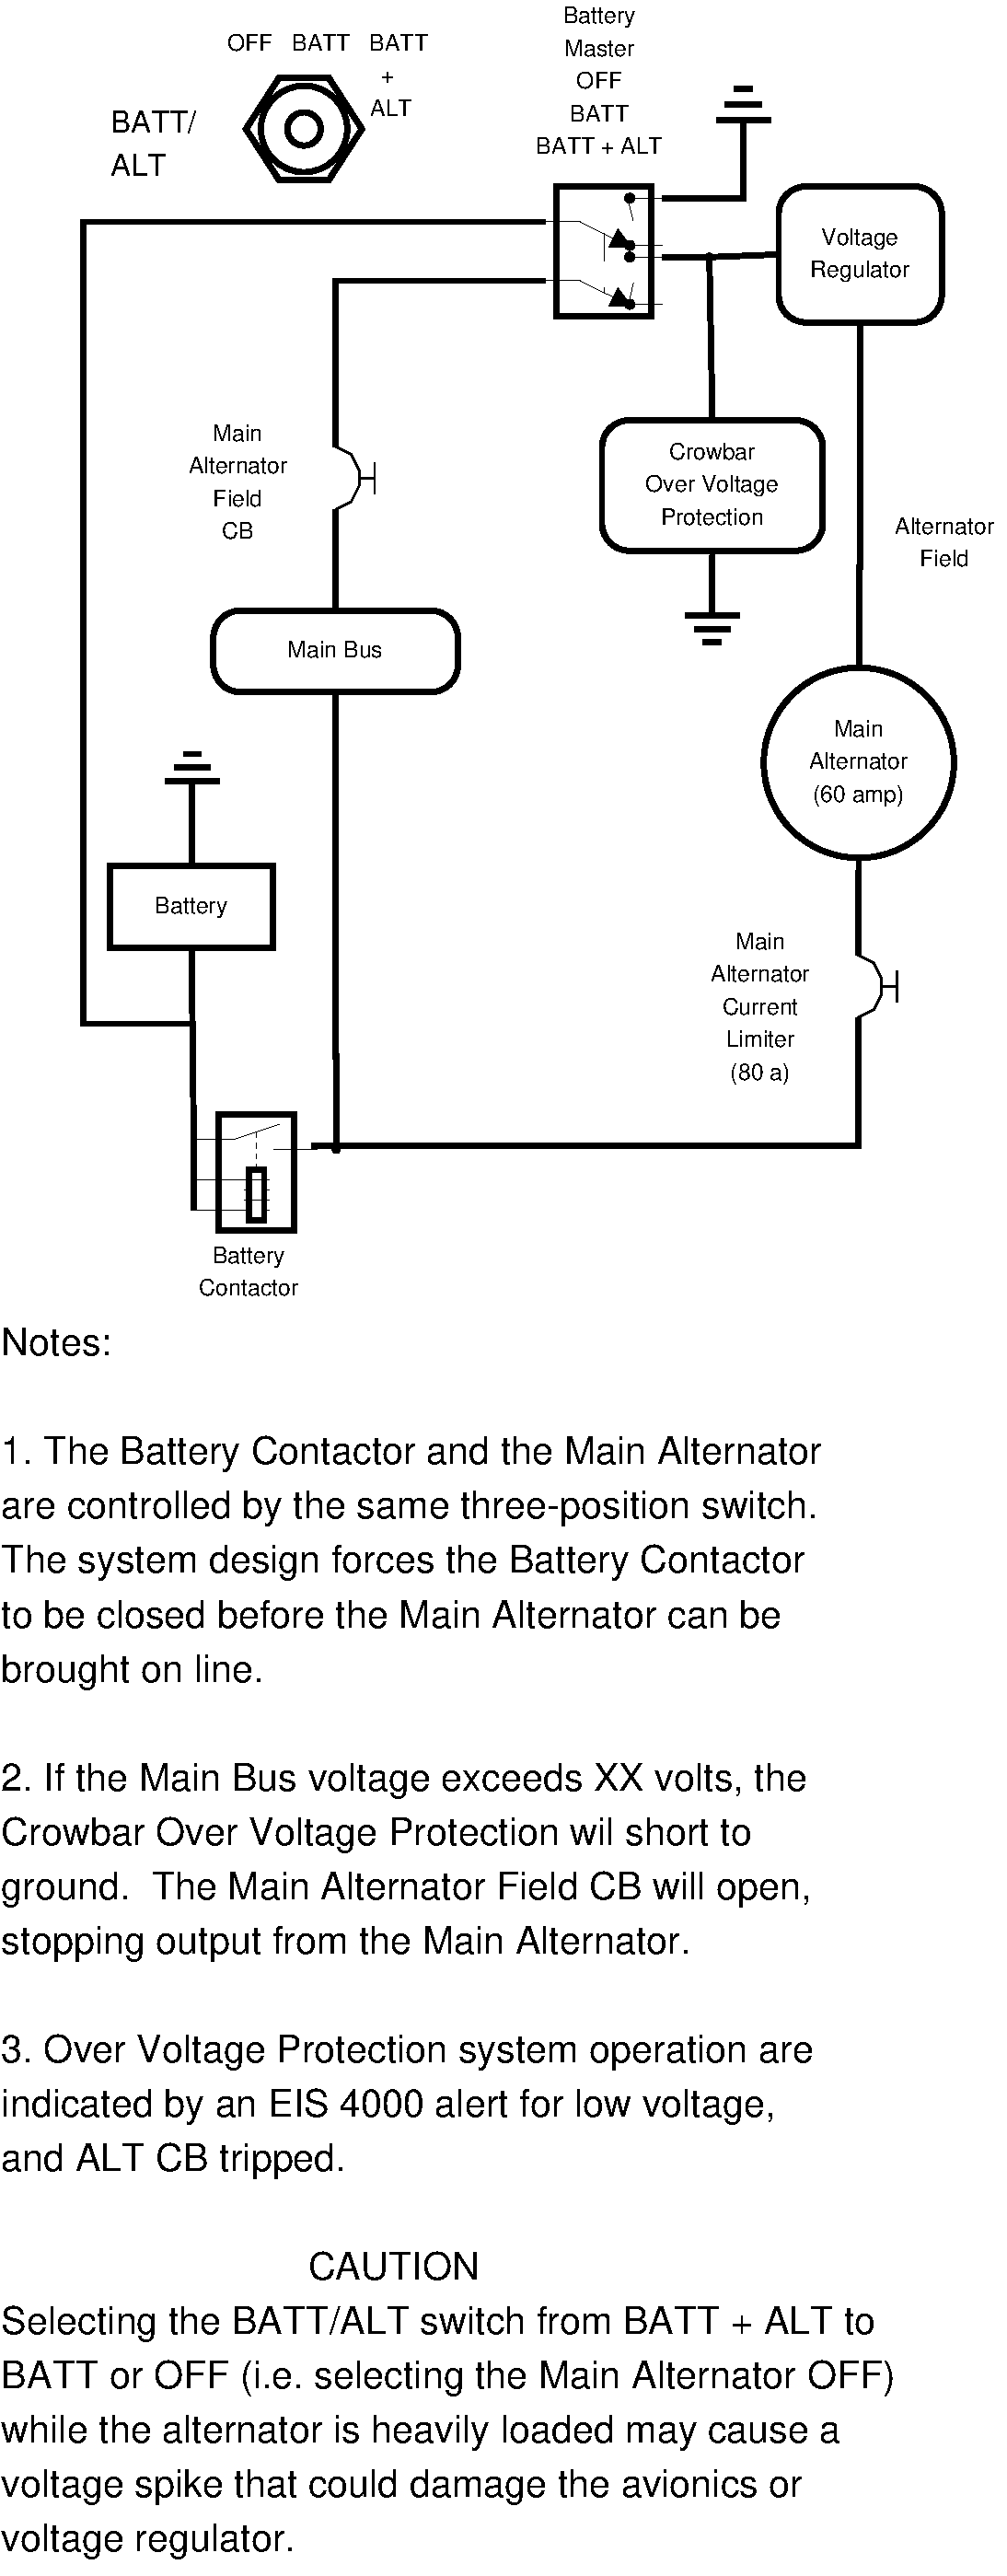
\includegraphics[scale=0.4]{../Diagrams/Alternator_large_note_narrow} \caption{Main Alternator Control} 
\end{figure}

\begin{figure}
\centering 
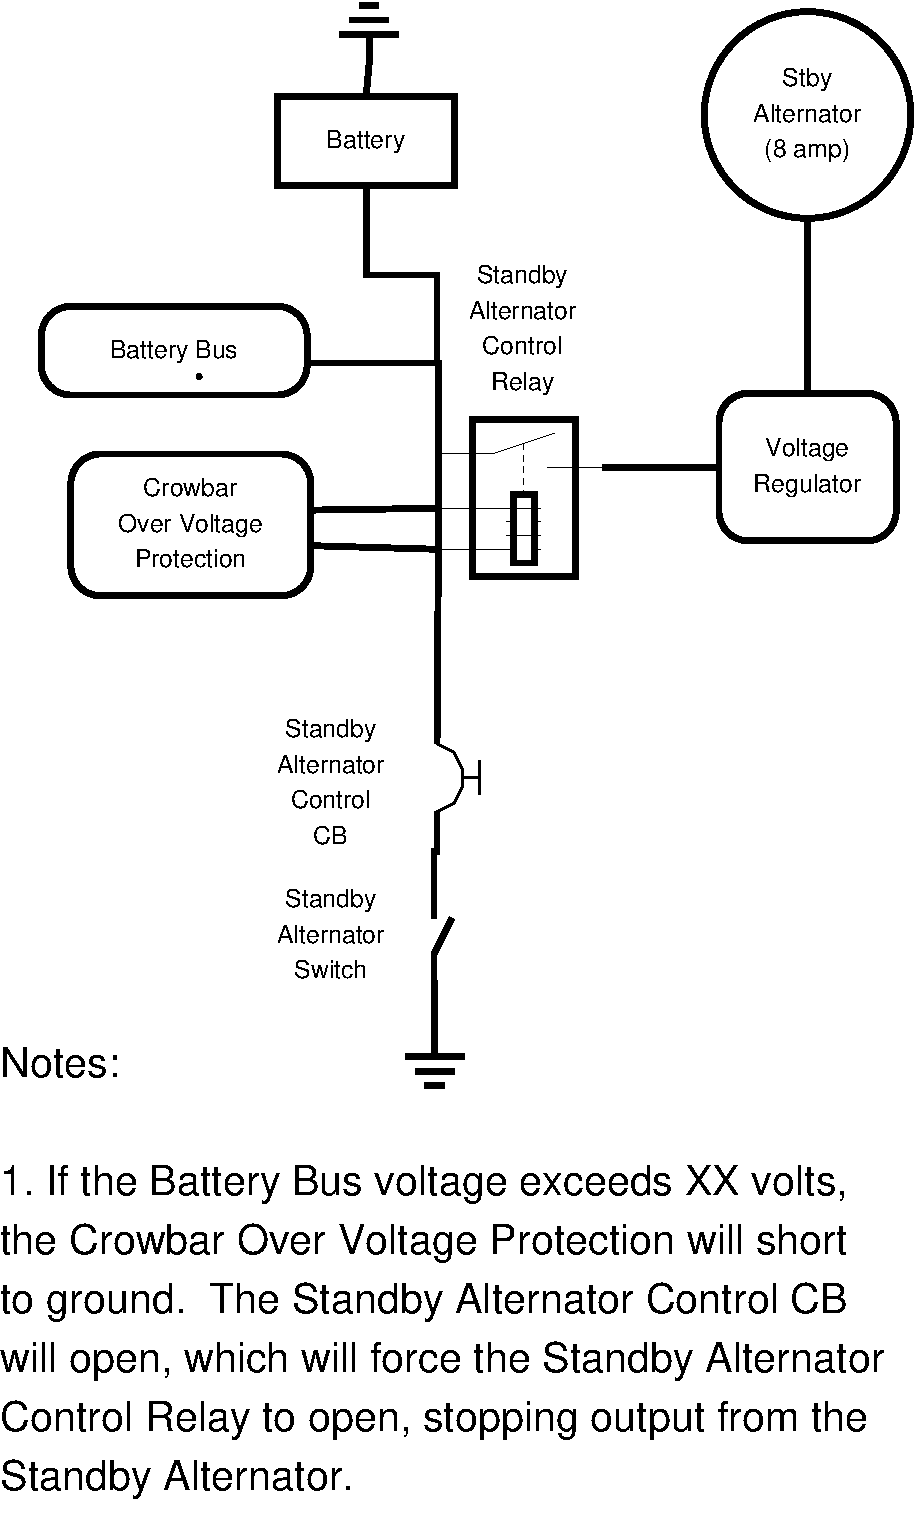
\includegraphics[scale=0.4]{../Diagrams/Alternator2_large_note_narrow} \caption{Standby Alternator Control}
\end{figure}

\textbf{Electrical System Switches} --- Electrical system switches are positioned on the right switch console. The master relay and the Main Alternator are controlled by the same three-position switch. The switch positions are OFF, BATT and BATT+ALT. The Standby Alternator can supply power to the Battery Bus, and the Essential Bus even if the BATT/ALT switch is selected to OFF.

\textbf{Over Voltage Protection} --- Each alternator has independent over voltage protection. If the alternator output voltage is too high, the over voltage protection system will short the Main Alternator field or the Standby Alternator relay to ground. This will open a CB on the aft end of the right side switch console, and shutdown the affected alternator. The over voltage protection may be reset by pushing the CB back in, but it will pop again if the over voltage condition still exists.

\textbf{Electrical System Circuit Protection} --- All circuit protection is by fuses, except for circuit breakers for the Main Alternator Field and the Standby Alternator Relay. The fuses for the Main and Essential busses are mounted on the aft face of the hinged door on the forward baggage compartment aft bulkhead, and are accessible on the ground only.  Battery Bus fuses are in a fuse block next to the battery, behind the aft baggage compartment. Fusible links are also used to protect some of the wires.

%\clearpage %force electrical system figures and table to appear, before moving on to next system
\begin{table}
[htb] 
\begin{center}
\begin{tabular}
{|l|l|l|} \hline \multicolumn{1}{|c|}{Main Bus}& \multicolumn{1}{c|}{Essential Bus} & \multicolumn{1}{c|}{Battery Bus}\tabularnewline \hline \hline EFIS Main Power & GNS 430W & Turn and Bank\tabularnewline \hline Microair COM &CDI & Electronic Ignition\tabularnewline \hline Narco 122D & Transponder & EFIS Emergency Power\tabularnewline \hline Audio Panel &Grand Rapids EIS 4000 & Aux Power Outlet\tabularnewline \hline CO Monitor &Inst. Panel Lighting & \tabularnewline \hline Engine Inst. Lighting &Goose Neck Flood Light & \tabularnewline \hline CDI Lighting &Pitch Trim & \tabularnewline \hline Landing Light &Roll Trim & \tabularnewline \hline Taxi Light &Fuel Gauges & \tabularnewline \hline Position Lights &ELT GPS Decoder & \tabularnewline \hline Strobe Lights & & \tabularnewline \hline Oil Press. Warning Light & & \tabularnewline \hline Starter & & \tabularnewline \hline Flaps & & \tabularnewline \hline Boost Pump & & \tabularnewline \hline Pitot Heat & & \tabularnewline \hline Autopilot & & \tabularnewline \hline Hour Meter & & \tabularnewline \hline Tachometer & & \tabularnewline \hline Manifold Pressure Gauge & & \tabularnewline \hline Defog Fan & & \tabularnewline \hline 
\end{tabular}
\caption{Items Powered By Each Electrical Bus} 
\end{center}
\end{table}

%\textcolor{red}{Add fuse block table}
\begin{sidewaysfigure}
\centering 
% 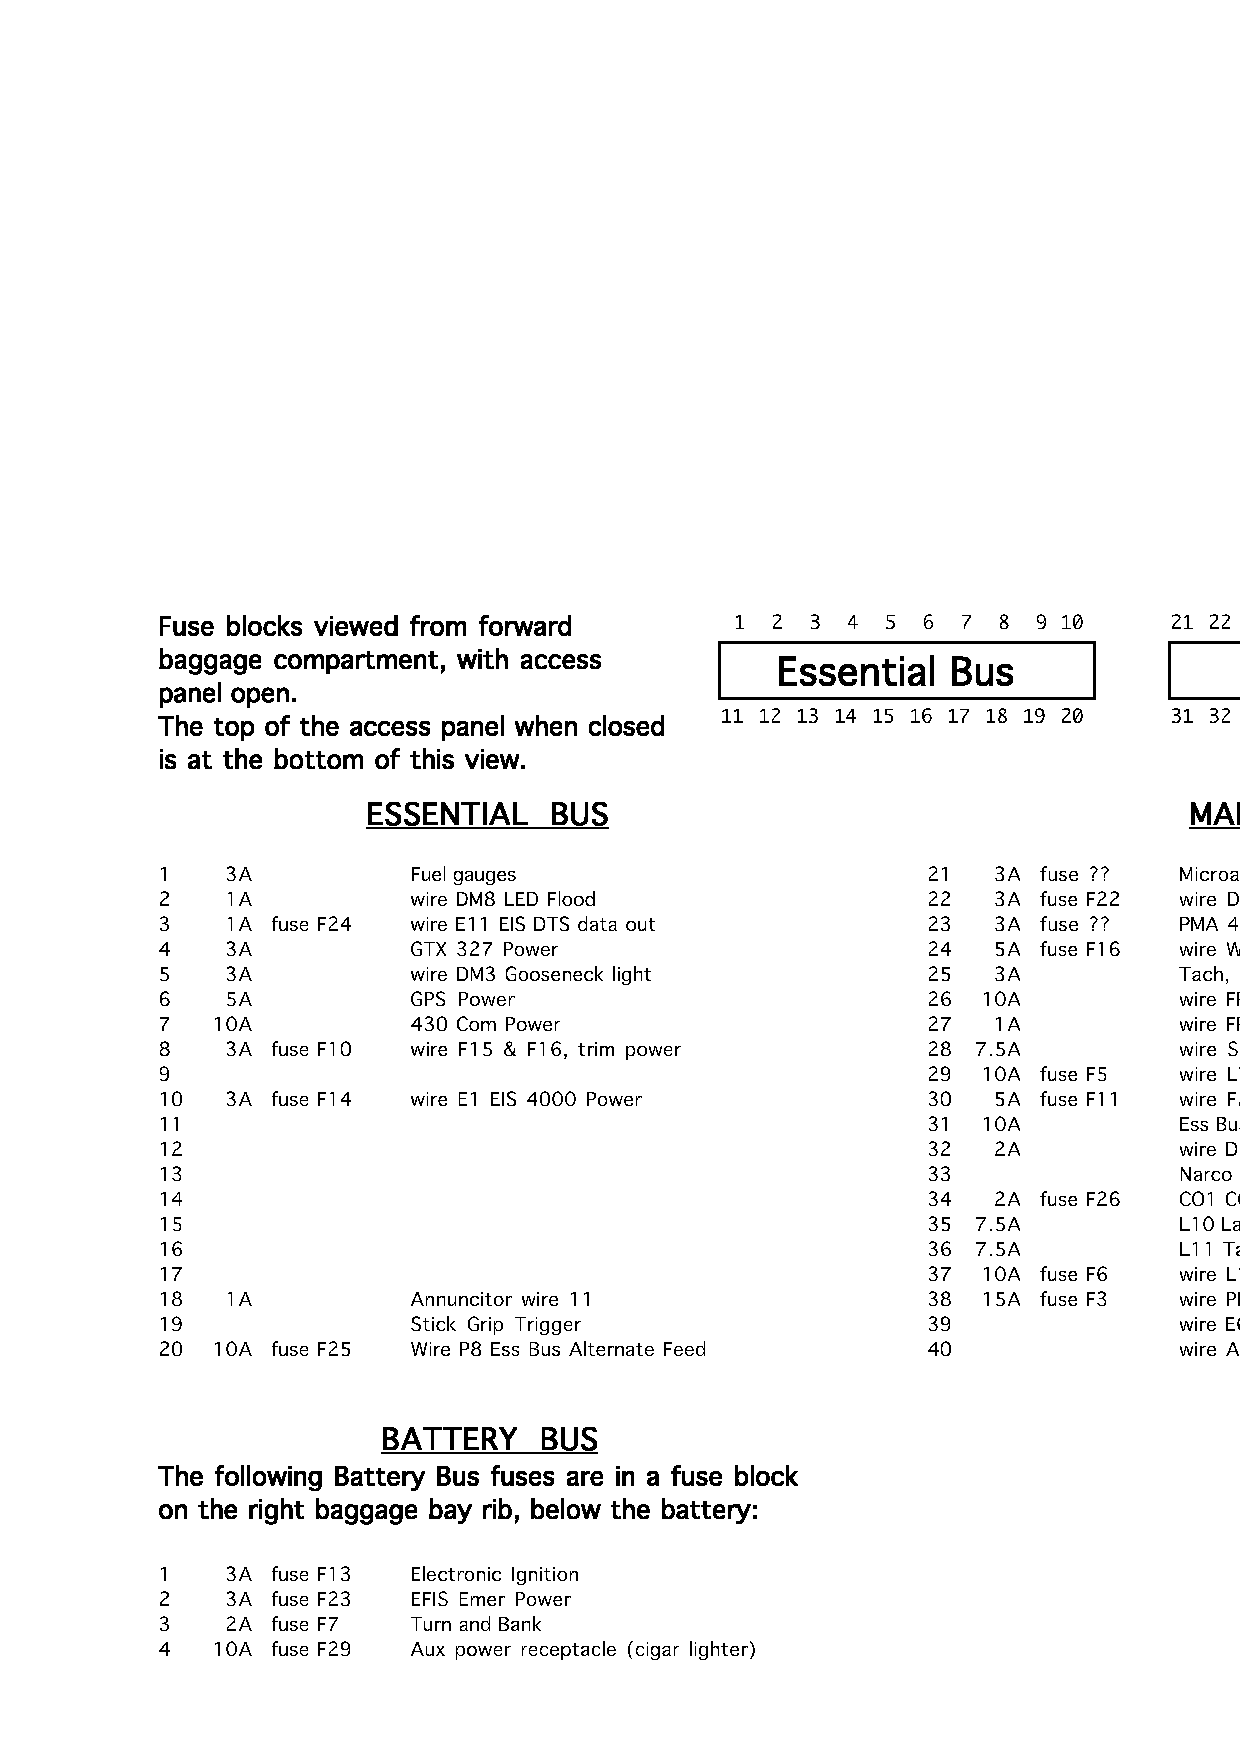
\includegraphics[width=\textwidth, scale=0.5]{../Diagrams/fuse_blocks} \caption{Fuse Locations}
% 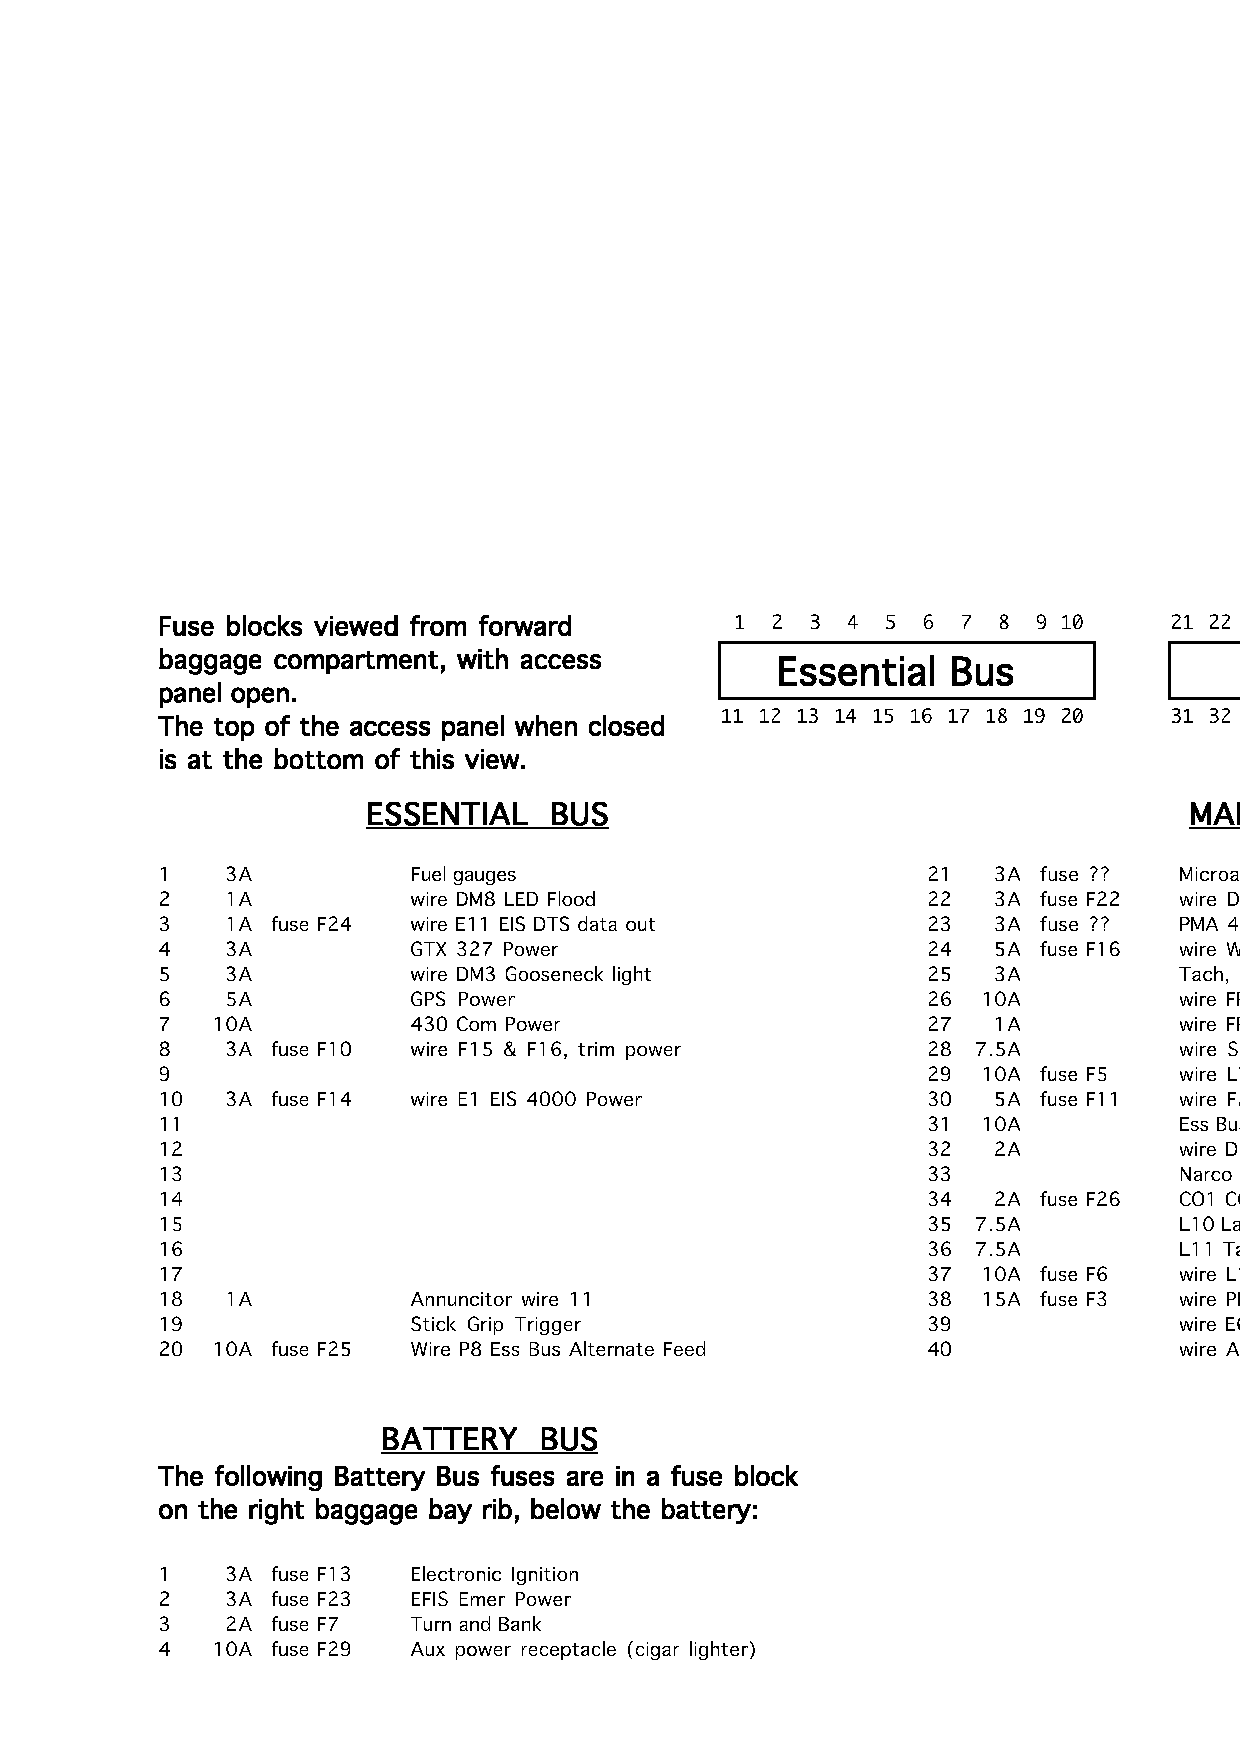
\includegraphics[scale=0.8]{../Diagrams/fuse_blocks} \caption{Fuse Locations}
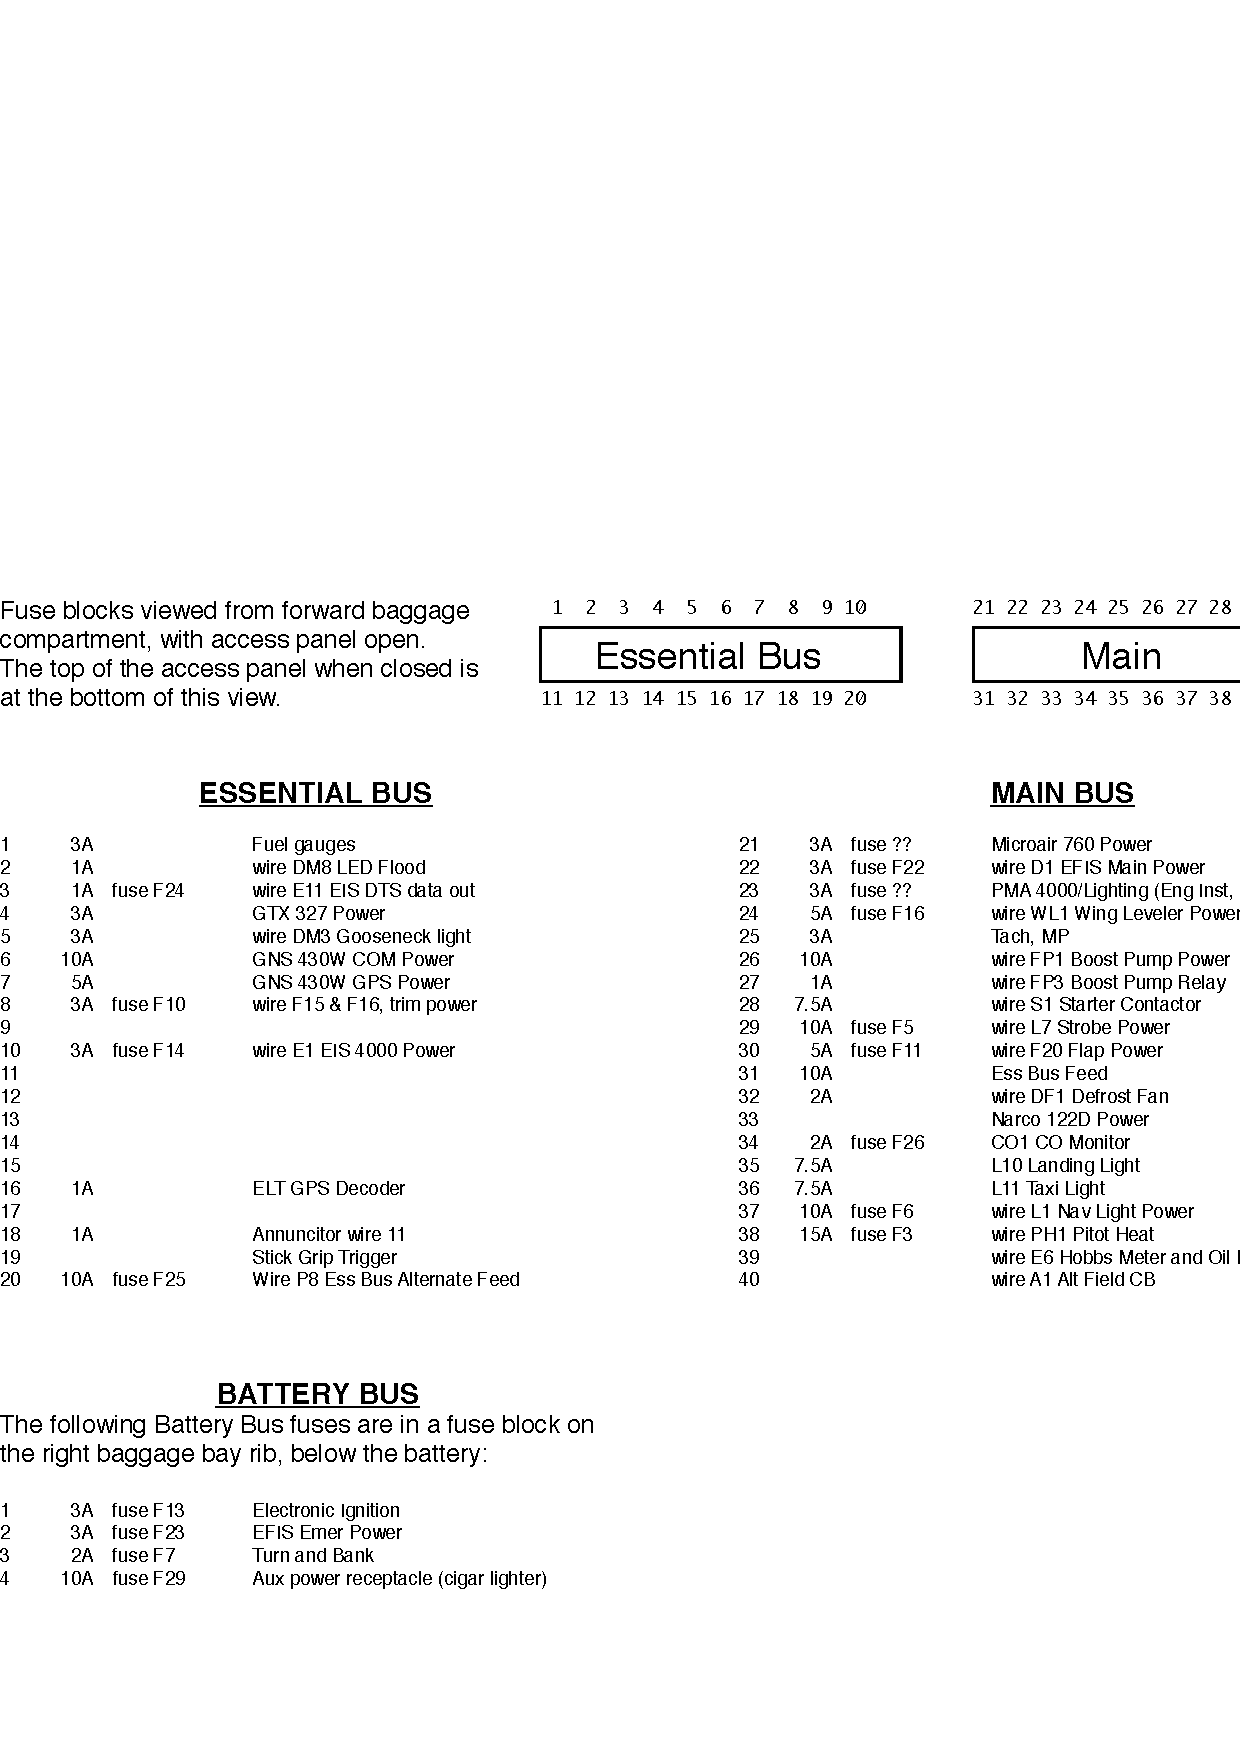
\includegraphics[scale=0.8]{../Diagrams/Fuse_Blocks_POH} \caption{Fuse Locations}


\end{sidewaysfigure}

\FloatBarrier

\section{COCKPIT LIGHTING}

\textbf{PANEL FLOOD LIGHTS} --- The main instrument panel lighting is provided by two white LED flood lights, one mounted on the front end of each canopy sill. The flood lights are powered from the Essential Bus, and are controlled by the left-most dimmer knob on the lower left part of the main instrument panel, labelled ``INST PANEL''.

\textbf{GOOSE-NECK FLOOD LIGHT} --- Map lighting and emergency instrument panel lighting is provided by a goose-neck lamp mounted on the right wall of the front cockpit, powered from the Essential Bus. It is controlled by a dimmer knob fitted next to the base of the lamp. The goose-neck may be removed from the socket by pressing the release button next to the base.

\textbf{760 COM DISPLAY} --- The display back-lighting for the Microair 760 COM is controlled by the INST PANEL dimmer knob. The display back-lighting is powered even if the 760 COM is unpowered.

\textbf{GARMIN GNS 430W \& GTX 327} --- The display and key back-lighting for the Garmin GNS 430W GPS and GTX 327 Transponder are controlled by the middle dimmer knob, labelled ``AVIONICS''. The display intensity is controlled by an ambient light sensor if the dimmer knob is rotated fully counter clock-wise --- this allows the display intensity to increase as required in bright sunlit conditions.

\textbf{ENGINE INSTRUMENTS \& CDI} --- The analog tachometer, manifold pressure, fuel gauges and CDI are internally lit --- these lights are powered from the Main Bus. The light intensity is controlled by the right-most dimmer knob, labelled ``CDI + ENG INST''. 

\section{EXTERNAL LIGHTING}

\textbf{Landing Light} --- The Landing Light is installed in the right outboard wing. It is powered from the Main Bus and uses a 55 amp halogen automotive bulb. The switch is on the left side of the instrument panel. 

\textbf{Taxi Light} --- The Taxi Light is installed in the left outboard wing, and is identical to the landing light, except it is aimed at a lower angle. It is powered from the Main Bus, and its switch is on the left side of the instrument panel.

\textbf{Flash Function} --- The Landing and Taxi Lights also have a ``wig-wag'' flash function which flashes the two lights alternately. It is selected by placing both the Landing and Taxi Light switches in the middle, ``FLASH'' position.

\textbf{Position Lights }- The aircraft is fitted with red, green and white position lights in the left wing tip, right wing tip and rudder bottom respectively. The wing tip position lights are mounted under flush covers in the forward edge of the wing tips. The rudder bottom light is in the centre of a concentric position light/strobe light assembly. The position lights are powered from the Main Bus, and the switch is located on the left side of the instrument panel. The switch has three positions: ``OFF'', ``NAV'', and ``NAV + STR''. The position lights are ON if the switch is in either of the latter two positions.

\textbf{Strobe Lights} --- The aircraft is fitted with white strobe lights, with strobe tubes under flush covers on each wing tip and on the aft end of the rudder bottom fairing. The strobe lights are powered from the Main Bus, and the switch is located on the left side of the instrument panel. The switch has three positions: ``OFF'', ``NAV'', and ``NAV + STR''. The strobe lights are ON only if the switch is in the ``NAV + STR'' positions.

\section{PITOT-STATIC SYSTEM}

The pitot system provides pitot pressure to the EFIS and the airspeed indicator. The heated pitot tube is located under the left wing, about two thirds of the way along the span. The pitot heat, powered from the Main Bus, is controlled by the PITOT HEAT switch on the right hand console.

The static system supplies static pressure to the EFIS, airspeed indicator, altimeter, vertical speed indicator and altitude encoder (which provides altitude information to the transponder). The static pressure ports are on the rear sides of the fuselage and are positioned to self drain. An alternate static port is located near the bottom of the right landing gear box in the cockpit. The alternate static port is a locking valve which is spring loaded closed. It can be pushed upwards and turned to lock it in the open position. Airspeed and altitude corrections must be applied if the alternate static port is open. 

\section{HEATING AND VENTILATION}

Cabin heat is provided via two heat muffs attached to the exhaust system and fed with high pressure air taken from the baffling behind \#3 cylinder and ahead of \#1 cylinder. The heated air is ducted through the firewall in two locations: ahead of the rudder pedals, and on the rear wall of the front baggage compartment lower extension, near the right landing gear box. The heat is controlled by two push/pull cables just below the right heat outlet. The right heat outlet is from an orientable eyeball vent that may be pointed to blow the hot air past the right side of the pilot towards the passenger.

Ventilation air is supplied from two NACA inlets: one on the front left side of the fuselage for the pilot, and one under the right wing for the passenger. The pilot's ventilation air is fed to an eyeball vent under the left side of the instrument panel. The passenger's ventilation air is fed to an eyeball vent just aft of the front seat back.

A Defog Fan is mounted beneath a grill on the glare shield. It is controlled by a switch on the right console, and blows air from under the instrument panel against the windscreen.
\clearpage 
\section{DYNON D-10A EFIS} 
\piccaption{Dynon D-10A EFIS} 
\parpic[r]{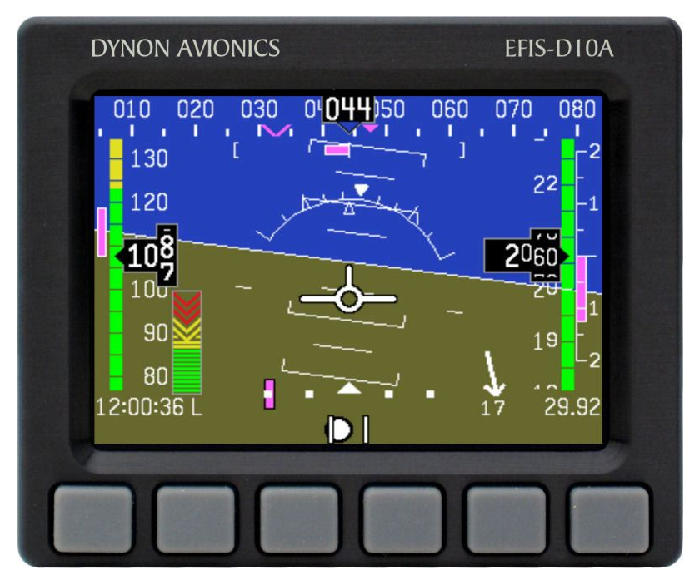
\includegraphics[scale=0.65]{../Diagrams/d10a_new_format}}

The Dynon D-10A EFIS provides attitude, heading, airspeed, altitude, vertical acceleration and slip ball information on a 4" colour LCD display.

\textbf{Operator Interface} --- The six buttons along the bottom of the bezel provide access to various functions. After a button is pushed, labels are displayed above each button. The far-right button will always command a return to the previous menu.

\textbf{Power} --- The EFIS is normally powered from the Main Bus. The unit may be turned ON by pressing the far-left button. If Main Bus power is lost, the unit will automatically transition to its internal battery for 30 seconds, then shutdown. A screen message will be displayed, warning of the impending shutdown. This automatic shutdown may be cancelled by pressing the far-left button.

If Main Bus power is lost, but aircraft battery power is still available, the EFIS BU switch on the right console may be selected to provide EFIS power from the Battery Bus.

If any power source is lost, an on-screen voltmeter display will appear, showing the voltage levels of the EFIS main power, emergency power and internal battery.

The unit may be turned OFF by pressing the holding the POWER button, which is the far-left button on the Main Menu.

\textbf{Attitude} --- The EFIS uses solid-state accelerometers and rate gyros to determine the attitude. Airspeed data is used to provide acceleration corrections, so the attitude info may be in error during manoeuvring if the pitot or static lines are blocked. The attitude information may become invalid for short periods following extreme manoeuvres (e.g. aerobatics or spins). The colours of the attitude display will be changed from the normal blue/brown to shades of grey if the EFIS detects that the displayed attitude may not be valid.

\textbf{Heading} --- The heading is sensed by a remote flux valve mounted in the rear fuselage. The flux valve may be affected by the steel canopy frame when the canopy is open. It is possible that EMI from the flux valve may be heard on the COM. The flux valve may be disabled by selecting the ``FLUX VALVE'' switch OFF on the upper left side of the instrument panel. If the flux valve is disabled, the unit will use an internal flux valve, but it has very large errors, so the heading info will be essentially meaningless.

\textbf{Altimeter Setting} --- The altimeter setting can be viewed or changed via the BARO selection from the Main Menu.

\textbf{Bugs} --- Airspeed, altitude and heading bugs may be set via the BUGS selection from the Main Menu.

\textbf{Dimmer} --- Screen intensity can be set via the DIM selection on the Main Menu 2 page {[}Main Menu $\Rightarrow$ MORE $\Rightarrow$ DIM{]}.

\textbf{Optional Display Items} --- The CLUTTR menu item allows the user to select which items are displayed {[}Main Menu $\Rightarrow$ MORE $\Rightarrow$ SETUP $\Rightarrow$ CLUTTR{]}. For example, the airspeed vertical tape and digital readouts may be independently selected, if desired. 

The INFO menu controls optional VSI, voltmeter and accelerometer displays {[}Main Menu $\Rightarrow$ MORE $\Rightarrow$ INFO $\Rightarrow$ LEFT (or RIGHT, as desired){]}.

Information on the following additional, optional functions may be found in the EFIS Pilot's User Guide:

\begin{itemize*}
\item Timer 
\item Clock 
\item G-meter 
\item VSI 
\item Turn Rate Display 
\item Checklists (not currently programmed)
\item HSI (not currently configured for display)
\end{itemize*}

\section{GARMIN GNS 430W GPS/NAV/COM} 
\begin{figure}
[htb] 
\begin{center}
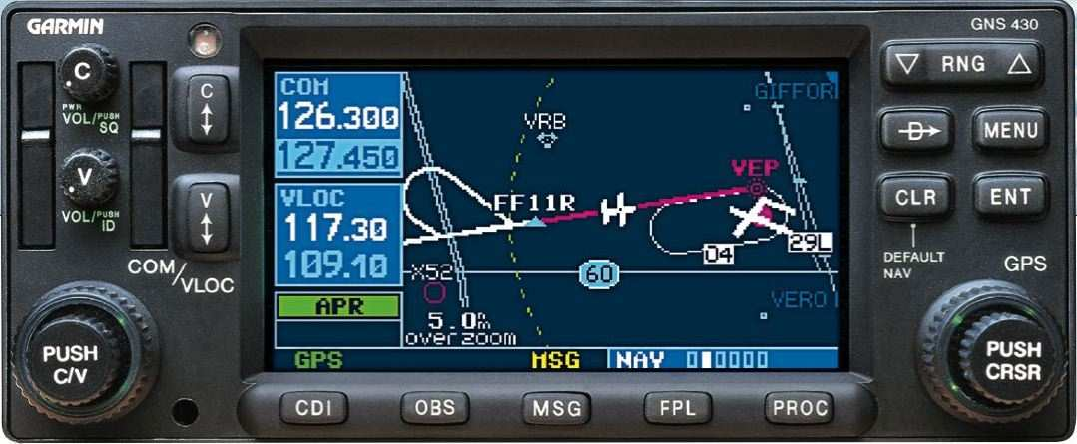
\includegraphics[scale=0.8]{../Diagrams/gns430_1}
\end{center}
\caption{Garmin GNS 430W} 
\end{figure}

This section will only provide info on basic functions required for VFR flight. See the Garmin GNS 430W Pilot's Guide and Reference for more detailed information, and coverage of IFR related functions. Some aspects of the functionality are configurable via configuration menus (see Pilot's Guide for details).

The GNS 430W System is a fully integrated, panel mounted instrument, which contains a VHF Communications Transceiver, a VOR/ILS receiver, and a Wide Area Augmentation System (WAAS) Global Positioning System (GPS) Navigation computer. The system consists of a GPS antenna, GPS Receiver, VHF VOR/LOC/GS antenna, VOR/ILS receiver, VHF COMM antenna and a VHF Communications Transceiver. 

Provided the Garmin GNS 430W's GPS receiver is receiving adequate usable signals, it has been demonstrated capable of and has been shown to meet the accuracy specifications for:
\begin{enumerate}
\item VFR/IFR enroute, terminal, and non-precision instrument approach (GPS, VOR, VOR-DME, NDB, NDB-DME, RNAV) operation using WGS-84 (or NAD 83) coordinate reference datum in accordance with AC 20-138. \textcolor{red}{Add WAAS info.}
\item The system meets RNP5 airspace (BRNAV) requirements of AC 90-96 and in accordance with AC 20-138, and JAA GAI-20 ACJ 20X4, provided it is receiving usable navigation information from the GPS receiver. 
\item The equipment as installed has been found to comply with the requirements for GPS primary means of navigation in oceanic and remote airspace, when used in conjunction with the 400 Series Trainer Program incorporating the FDE Prediction Program. This does not constitute an operational approval. 
\end{enumerate}
Navigation is accomplished using the WGS-84 (NAD-83) coordinate reference datum. Navigation data is based upon use of only the Global Positioning System (GPS) operated by the United States of America.

The GNS 430W provides GPS, COM, VOR, LOC and G/S capability with a colour moving map display. The COM is connected to the COM 1 on the audio panel. The CDI may display either GPS, VOR or ILS info.

\textbf{Power} --- The GNS 430W is powered from the Essential Bus. The unit is turned ON/OFF by turning the COM PWR/VOL switch at the top left corner. The Self-Test page data must be verified for IFR navigation using the GPS.

\textbf{COM} --- The GNS 430W COM is connected to the COM1 selection of the Audio Panel. The COM volume is controlled by the PWR/VOL knob at the top left corner. This knob is pushed to toggle the squelch ON/OFF. Two concentric tuning knobs at the lower left select the standby frequency for the COM and NAV. The frequency tuning function will default to COM, but it may be toggled between the COM and NAV functions by pushing the inner tuning knob (marked ``PUSH C/V''). The standby and active frequencies are exchanged by pushing the ``C$\updownarrow$'' button.  Press and hold the ``C$\updownarrow$'' button to switch to 121.5 mHz.

\textbf{NAV} --- The frequencies are tuned as described in the COM section. The NAV audio may be selected via the audio panel. The NAV volume is controlled by the lower of the two VOL knobs (marked ``V''). The NAV idents are not fed to the NAV audio by default, but they may be selected by pushing the NAV volume knob.

\textbf{CDI} --- the external CDI nav source is selected to either GPS or NAV by the CDI button on the bottom bezel. The current CDI nav source is indicated above the CDI button and by a lit indication on the CDI itself. If GPS is the nav source, the CDI scaling is indicated above the CDI button (see Table \ref{cdi} below).

\begin{Note}
\centering
The internal CDI display on the NAV 1 page always shows GPS information.
\end{Note}
\raggedright

\begin{table}
[htb] 
\begin{center}
\begin{tabularx}
  % {\textwidth}{|>{\setlength\hsize{.5\hsize}}Y|c|>{\setlength\hsize{1.5\hsize}}Y|} \hline Annunciation&Meaning\\
  {\textwidth}{|c|X|c|} 
  \hline ANNUNCIATION&MEANING&APPROACH\tabularnewline
  &&MINIMUMS\\
	\hline
	\hline DPRT & Departure, indicates the system is using non- precision approach integrity. HAL = 0.3 and CDI full-scale deflection is 0.3 NM.&\\
	\hline ENR & En route, CDI full-scale deflection is 2.0 NM or current CDI scale selection, whichever is smaller.&\\
	\hline TERM & Terminal, CDI full-scale deflection is 1.0 NM or current CDI scale selection, whichever is smaller.&\\
	\hline LNAV & GPS approach active. &LNAV\\
	\hline LNAV+V & GPS approach active + advisory baro vertical guidance.&LNAV\\
	\hline L/VNAV & Lateral Navigation and Baro Vertical Navigation (LNAV/VNAV) approach active. &LNAV/VNAV\\
	\hline LP & LP indicates Localizer Performance active with no vertical guidance.&LP\\
	\hline LPV & Localizer Performance with Vertical guidance (LPV) approach active.	A yellow background indicates that the approach is safe to continue but a downgrade to LNAV may occur.&LPV\\
	\hline MAPR & Missed Approach indicates the system is providing missed approach integrity and CDI full-scale deflection $\pm $0.3 NM.&\\
  \hline LOW ALT & For LNAV+V, LNAV/VNAV, or LPV approaches, the LOW ALT annunciation indicates the aircraft's estimated height is significantly lower than the Final Approach Waypoint height.&\\
	\hline
\end{tabularx}
\caption{CDI Scaling Indications} \label{cdi}
\end{center}
\end{table}

\textbf{GPS Direct-To} --- For GPS Direct-To navigation, push the \directto button. Dial up the identifier using the inner right knob to select characters, and the outer right knob to move to the next character. Press ENT when the identifier is complete. Press ENT again to activate.

\textbf{Colour Moving Map Display} --- Press the CLR button to go to the default NAV page (CDI type display plus digital nav data). Rotate the inner right knob one click to the right to get to the moving map display. The range is changed with the Range rocker switch at the top right of the unit.

\textbf{Nearest Airports} --- Rotate the right outer knob all the way to the right, to display the NRST pages. Rotate the inner right knob all the way to the left to the Nearest Airports page. The three nearest airports are displayed, with six additional near airports available if the page is scrolled. The page may be scrolled by pushing the right inner knob to enable the cursor, then rotating the right inner knob to move the cursor. Direct-to navigation may be selected to an airport by moving the cursor to the airport identifier, then pressing the \directto button.

The airport tower or traffic frequency may be moved to the COM standby position by moving the cursor to the desired frequency on the NRST page and pressing the ENT button. Press the ``C$\updownarrow$'' button to exchange the standby and active COM frequencies.

\textbf{Antennae} --- The GPS/WAAS antenna is mounted on the upper fuselage immediately behind the passenger seat. The COM antenna is mounted on the left side of the bottom of the fuselage just behind the wing main spar. The NAV antenna is mounted inside the right wing tip. The signal from the NAV antenna also provides glide slope info.

\section{MICROAIR 760 COM} 
\piccaption{Microair 760 COM} 
\parpic[r]{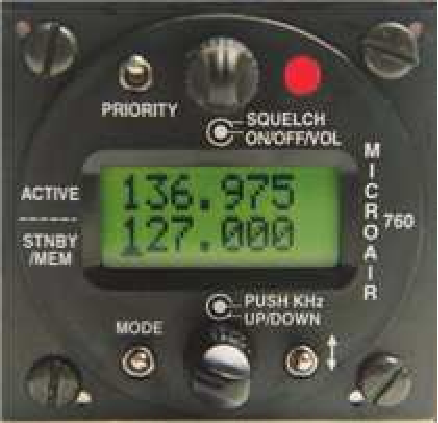
\includegraphics[scale=0.842]{../Diagrams/microair}}


The Microair 760 COM radio is positioned in a 2 1/8" instrument hole on the upper left side of the instrument panel above the GNS 430W, and is connected to the COM2 position of the Audio Panel.

\subsection*{Controls and Indicators}

\textbf{PRIORITY} --- Top left. A momentary down push selects the frequency in Memory 25, which is 121.5 MHz by default.

\textbf{ON/OFF/VOL} --- Inner top knob. Controls power and volume. 

\textbf{SQUELCH} --- Outer top knob.

\textbf{Annunciator LED} --- Top right. Indicates:

\begin{tabular}{lp{2.9in}} 
Red (steady)&Radio is transmitting\\
Red (flashing)&Radio has transmitted for longer than 30 seconds.\\
Green&A signal is received, or the squelch is set so background static is heard.\\
Off&Radio is not receiving a signal, and the squelch is set so background static is not heard.\\
\end{tabular}

\textbf{MODE} --- Bottom left. Momentary down pushes on the Mode toggle cycle the 760 COM thru the four modes of frequency selection. 
\begin{enumerate}
\item \textbf{Flip-Flop Mode} --- Flip-Flop mode has an active/standby functionality, with the active frequency displayed above the standby one. The standby frequency is changed using the bottom knob. Push the knob momentarily to switch the control between MHz and KHz. The control defaults to MHz after five seconds of inactivity. An underline cursor indicates the field that is currently selected. The active and standby frequencies are exchanged by making a momentary down movement on the $\updownarrow$ toggle. 
\item \textbf{Memory Mode} --- The top line displays ``MEM XX'', where ``XX'' is the memory number. The lower line displays the frequency in that memory location. The available frequencies are scrolled by rotating the frequency knob (lower knob). A frequency becomes active the moment it is displayed. 
\item \textbf{Program Mode} --- Used to program the frequencies stored in the current memory location. The top line displays ``PROG XX'', where ``XX'' is the memory number. The frequencies in each memory location may be changed. Lower knob changes frequency and memory number (momentary press of knob cycles it between MEM, MHz and KHz). The frequency is stored by a momentary press of the $\updownarrow$ toggle. The memory location is cleared by pressing and holding the Priority switch 
\item \textbf{Scan Mode} --- Scan mode is selected by pressing and holding the Priority toggle for three seconds. The radio cycles through the memory frequencies, stopping for 10 seconds on each frequency that has a signal. Scan operation is terminated by a momentary press of the $\updownarrow$ toggle, or the PTT switch. 
%\item \textbf{Priority Switch} --- A momentary down push on the Priority toggle selects the frequency in Memory 25, which is 121.5 MHz by default. 
\end{enumerate}

\subsection*{Other}

\textbf{Power Source} --- The 760 COM is powered from the Main Bus.

\textbf{Back-lighting} --- The display back-lighting intensity is controlled by the \textcolor{red}{INST PANEL} dimmer.

\textbf{Antenna} --- The 760 COM is connected to an antenna inside the left wing tip. 

\section{NARCO 122D VOR/ILS}
\piccaption{Narco 122D} 
\parpic[r]{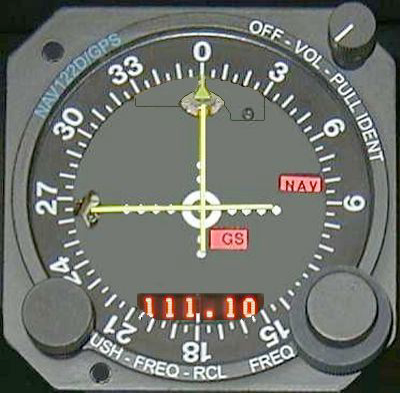
\includegraphics[scale=0.92]{../Diagrams/Narco122D_large}}


The Narco 122D is a VOR/ILS receiver with an integral CDI display. It is located at the lower, centre part of the instrument panel, directly below the CDI. The Narco 122D is \textbf{not} connected to the audio panel, so it is not possible to listen to navaid idents. 

\subsection*{Controls and Indicators}

\textbf{OFF --- VOL --- PULL IDENT} --- Top right. Controls power. The 122D is not connected to the audio panel, so the VOL and PULL IDENT functions are inoperative.

\textbf{FREQ} --- Bottom right. Inner and outer concentric knobs to select the VOR or ILS frequency.

\textbf{Course Select} --- Unlabelled knob at bottom left. Selects the desired course.

\subsection*{Other}

\textbf{Power Source} --- The Narco 122D is powered from the Main Bus. 

\textbf{Back-lighting} --- The Narco 122D has no internal backlighting.  It is illuminated by the instrument panel flood flights.

\textbf{Antenna} --- The Narco 122D receives NAV and G/S signals from the same antenna that feeds the GNS 430W, which is mounted inside the right wing tip.

\clearpage 
\section{AUDIO PANEL} 
\piccaption{PMA-4000 Audio Panel} 
\parpic[r]{
\includegraphics[scale=1]{../Diagrams/pma4000}}

The PS Engineering PMA-4000 Audio Panel is located at the bottom of the avionics stack on the left side of the instrument panel.

\subsection*{Controls}

\textbf{Audio Selector Switches} --- Top. The four square audio selector switch are labelled as follows: 
\begin{itemize}
\item ``C1'' COM 1 --- GNS 430W COM 
\item ``C2'' COM 2 --- Microair 760 COM 
\item ``N1'' NAV 1 --- GNS 430W NAV audio 
\item ``N2'' NAV 2 --- not used. 
\end{itemize}

The switches are lit when selected (pressed in). The COM that is selected for transmission is also automatically selected for audio. Both the pilot and passenger may transmit. Only the person who pushes the PTT is heard on the transmission.

\textbf{Transmit Selector} --- Bottom left. The COM radio to be used for transmission is selected by the ``Com 1/Com 2'' toggle switch.

\textbf{Mode Selector} --- Bottom centre. The audio panel mode of operation is selected with the ``Iso/All/Off'' toggle. The modes work as follows: 
\begin{itemize}
\item \textbf{Iso} --- Pilot is isolated from the intercom and music audio. The pilot only hears the Com audio (and transmission side tone). The passenger hears only himself on the intercom and the music. 
\item \textbf{All} --- Both pilot and passenger hear intercom, radios and music. The music is automatically muted when the intercom is used. 
\item \textbf{Off} --- The audio power is not powered. The pilot is automatically directly connected to Com 1 transmission and reception, regardless of the switch selections. 
\end{itemize}

\textbf{Volume} --- Bottom right. The pilot's audio volume is controlled by the inner knob, labelled ``Pilot''. The passenger's volume is controlled by the outer knob, labelled ``Copilot''. \textcolor{red}{Headset volume controls too?}

\textbf{Squelch} --- There is no dedicated Squelch control. The audio panel processor continuously adjusts the squelch as required.

\textbf{PTT} --- The pilot's PTT is the black switch half-way up the left side of the stick grip. The rear seat PTT is the black button next to the headset jacks on the right cockpit side under the canopy sill.

\textbf{Hot Mike} --- Both pilot and passenger intercom are always in a ``hot mike'' configuration. 

\section{GARMIN GTX 327 TRANSPONDER}

The Garmin GTX 327 transponder is located below the GNS 430 on the left side of the instrument panel. It is supplied with pressure altitude data by an ACK A-30 altitude encoder. Some aspects of the functionality are configurable via configuration menus (see Pilot's Guide for details).
\begin{figure}
[htb] 
\begin{center}

\includegraphics[scale=0.8]{../Diagrams/GTX327}
\end{center}
\caption{Garmin GTX-327 Transponder} 
\end{figure}

\subsection*{Controls}

\textbf{ON} --- Selects Mode A. Transponder replies to interrogations, but does not report altitude.

\textbf{OFF} --- Turns off the transponder.

\textbf{STBY} --- Puts the transponder in standby mode. The altitude encoder is powered and starts warming up. 

\textbf{ALT} --- Selects Mode A and Mode C. Transponder responds to interrogations and reports altitude, if the altitude encoder has warmed up. The altitude encoder requires approximately seven minutes of power to warm up. 
%The transponder automatically switches from standby to ALT mode after takeoff, based on a ground speed signal from the GNS 430.

\textbf{IDENT} --- Sends an Ident pulse to the ground station for 18 seconds.

\textbf{VFR} --- Changes the code to 1200. Pressing VFR a second time returns the code to the previous value.

\textbf{0--7} --- Used to enter a new transponder code. Code selection is started by pressing a digit. The new code will not be activated until the fourth digit is entered. Pressing the CLR key will move the cursor back to the previous digit. Pressing the CRSR key will cancel code entry and return to the previous code.

\textbf{8--9} --- Used in Configuration Mode or to set the timer.

\textbf{FUNC} --- Changes the data shown on the right side of the display. Options are Pressure Altitude, Flight Time, Count-Up Timer, Count-Down Timer, Contrast and Display brightness. Note: the availability of Contrast and Brightness selections are controlled by a configuration menu.

\textbf{CRSR} --- Used to cancel code entry, and to enable the cursor to input the time for a Count-Down timer.

\textbf{$\mathrm{\frac{START}{STOP}}$} --- Starts and stops the count-up and count-down timers.

\textbf{CLR} --- Resets the count-up and count-down timers and cancels a key press during code entry.

\subsection*{Timers}

\textbf{Count-Up Timer} --- To operate the Count-Up Timer: 
\begin{enumerate}
\item Press the ``FUNC'' key until ``COUNT UP'' is displayed. 
\item If necessary, press ``CLR'' to reset the timer to zero. 
\item Press $\mathrm{\frac{START}{STOP}}$ to start the timer. 
\item Press $\mathrm{\frac{START}{STOP}}$ again to pause the timer. 
\item Press ``CLR'' to reset the timer to zero. 
\end{enumerate}

\textbf{Count-Down Timer} --- To operate the Count-Down Timer: 
\begin{enumerate}
\item Press the ``FUNC'' key until ``COUNT DOWN'' is displayed. 
\item Press the ``CRSR'' key and use the ``0--9'' keys to set the initial time. All digits must be entered, including leading zeros. 
\item Press $\mathrm{\frac{START}{STOP}}$ to start the timer counting down. 
\item Press $\mathrm{\frac{START}{STOP}}$ again to pause the timer. 
\item When the timer expires, the words ``COUNT DOWN'' are replaced with ``EXPIRED'', and the timer begins counting up and flashing. 
\item Press ``CLR'' to reset the timer to the initial value. 
\end{enumerate}

\subsection*{Other}

\textbf{Power Source} --- The GTX 327 transponder is powered from the Essential Bus.

\textbf{Back-lighting} --- The display back-lighting intensity is controlled by the Avionics dimmer.

\textbf{Antenna} --- The GTX 327 transponder antenna antenna is mounted on the right side of the bottom of the fuselage just behind the wing main spar. 

\FloatBarrier 

%\section{WING LEVELER} 

The Navaid Devices AP-1 Wing Leveler may be operated in Turn Coordinator mode or Wing Leveler mode. A horizontal red LED display indicates turn rate. In Wing Leveler mode, wing leveler and GPS tracking modes are available. The WING LVLR switch on the LH console controls power to the wing leveler system. The power to the servo may be temporarily interrupted by pressing and holding the red master disconnect switch on the pilot's control stick. There is a clutch in the system that will slip to allow the pilot to override the wing leveler if required. %As a last resort, there is a removable pin where the wing leveler push rod connects to the base of the pilot's control stick. 

\subsection*{Controls}
\begin{tabular}{p{0.5\linewidth}p{0.5\linewidth}}
\begin{minipage}[b]{\linewidth}
\begin{enumerate}
\item \textbf{TK$\bullet$TC$\bullet$WL} --- Selects the mode of operation --- Track (TK), Turn Coordinator (TC), or Wing Leveler (WL). In Track mode, the unit tracks the GPS or NAV/LOC signal from the GNS 430, whichever is selected as the GNS 430W CDI source. In Turn Coordinator Mode, the unit is not connected to the flight controls, and simply serves as a back-up Turn Coordinator. In Wing Leveler mode, the unit provides aileron inputs to maintain zero yaw rate, or to turn, as controlled by the Turn knob. 
\item \textbf{TRIM} --- Adjusts the reference from the built-in yaw gyro. Used if the wings are not level when the Turn knob is in the centre detent. 
\item \textbf{TURN} --- Commands turns when the unit is in Wing Leveler mode. 
\item \textbf{TRIM POTS} --- Used to set the gains during flight testing. Should not be adjusted except as part of a dedicated flight test program. 
\end{enumerate}
\end{minipage} 
&
\begin{minipage}[b]{\linewidth}
\begin{overpic}
[scale=.8]{../Diagrams/ap1} 
\Large 
\put(7,36){\ding{172}} 
\put(7,52.5){\ding{173}} 
\put(95.5,52.5){\ding{174}} 
\put(95.5,28.75){\ding{175}} 
\put(-1,59.75){\ding{176}} 
\put(79,81.25){\ding{177}} 
\put(82,.75){\ding{178}} 
\normalsize 
\end{overpic}
\caption{Wing Leveler}
\end{minipage}\\
\end{tabular}

\subsection*{Indicators} 
\begin{enumerate}
\setcounter{enumi}{4} 
\item \textbf{TURN RATE} --- Bar of red LEDs illuminate to indicate turn rate. The centre LED is illuminated at zero turn rate. The bar extends from the centre to indicate the magnitude and direction of the turn rate. 
\item \textbf{STANDARD TURN MARKERS} --- Triangles above the turn rate bar indicate a 3 deg/second turn rate. 
\item \textbf{SLIP BALL} --- Indicates lateral acceleration. 
\end{enumerate}

\subsection*{Power}

\textbf{MAIN POWER} --- The Wing Leveler power is controlled by the WING LVLR switch on the right switch console. The unit is powered from the Main Bus.

\textbf{SERVO DISENGAGE} --- The servo power supply may be interrupted by pressing and holding the red TRIM/WING LEVELER disable switch on the front stick grip. %If required, the linkage between the servo and the stick may be disconnected by pulling the ``Pip'' pin that is located at the bottom of the front stick, just above the fore and aft pivot.



\section{AUTOPILOT} 

The Trio Avionics Pro Pilot autopilot moves the ailerons and/or elevators to control the aircraft. The autopilot can follow the GNS 430W lateral flight plan, including procedure turns and GPS, RNAV or LPV approaches. The autopilot vertical capabilities include altitude hold, vertical speed hold, altitude preselect and LPV vertical path. A two line alphanumeric display provides detailed information to the pilot. The WING LVLR switch on the LH console controls power to the autopilot system. The power to the servos may be temporarily interrupted by pressing and holding the red master disconnect switch on the pilot's control stick. The autopilot does not control the pitch trim --- the aircraft must be reasonably well trimmed in pitch to allow the autopilot to control the aircraft without reaching the force limit provided by the servo slip clutch. %Each servo has a clutch that will slip to allow the pilot to override the wing leveler if required. %As a last resort, there is a removable pin where the wing leveler push rod connects to the base of the pilot's control stick. 

The autopilot control head is on the instrument panel below the turn and slip indicator. The pitch servo is behind the rear baggage compartment, and the roll servo is beneath the horizontal panel just ahead and to the right of the front seat. The autopilot is powered from the Main Bus. Power is controlled by the Wing Leveler switch on the right console and also by the On toggle switch located at the top centre of the control head.

\textbf{Altimeter Setting} --- The autopilot does not have a means to directly enter an altimeter setting. Instead, the current altitude is entered whenever the "BARO SET" message is displayed, which allows the system to determine the needed offset to the pressure altitude sensed from the static input.

\subsection*{Controls}
\begin{tabular}{p{0.5\linewidth}p{0.5\linewidth}}
\begin{minipage}[b]{\linewidth}
\begin{enumerate}
\item \textbf{Power Switch} --- Controls all power to the autopilot control head and servos. This switch is in series with the Wing Leveler switch on the right switch console.
\item \textbf{"H~NAV"} --- Engages or disengages the horizontal (i.e. roll) servo. A three second press and hold engages the autopilot in emergency left course reversal (180\textdegree \ left turn with altitude hold).
\item \textbf{"V~NAV"} --- Engages or disengages the vertical (i.e. pitch) servo. A three second press and hold engages the autopilot in emergency right course reversal (180\textdegree \ right turn with altitude hold).
\item \textbf{"H~MODE"} --- Cycles the horizontal mode between TRK (track), CRS (course) and INT (intercept) modes, if the display is currently showing horizontal mode info. If the autopilot display is currently showing vertical mode information, the first press of the "H~MODE" button replaces that with horizontal mode information.
\item \textbf{"V~MODE"} --- Cycles the vertical mode between ALT HOLD (altitude hold), AS/VS (airspeed/vertical speed), ALT SEL (altitude select) and BARO SET (adjust altitude for altimeter setting changes). If the autopilot display is currently showing horizontal mode information, the first press of the "H~MODE" buttons replaces that with vertical mode informational.
\item \textbf{Rotary Knob} --- Allows pilot input of values by rotation and then pushing to enter. For changes to selected altitude, one click = 100 ft. If the knob is pressed, then turned, one click = 1000 ft. For changes to selected track, one click = 1\textdegree.
\end{enumerate}
\end{minipage} 
&
\begin{minipage}[b]{\linewidth}
\begin{overpic}
[scale=.8]{../Diagrams/ProPilot5} 
\end{overpic}
\caption{Trio Pro Pilot Autopilot}
\end{minipage}\\
\end{tabular}

\subsection*{Indicators} 
\begin{enumerate}
\setcounter{enumi}{6} 
\item \textbf{H LED} --- Illuminates when the horizontal servo is engaged. 
\item \textbf{V LED} --- Illuminates when the vertical servo is engaged. 
\item \textbf{GPSS LED} --- Blinks when roll steering info from the GNS 430W is available, but not being used because the autopilot is not in TRK mode. Illuminates steady when the autopilot is following roll steering info from the GNS 430W. The autopilot must be in TRK mode to use GPSS.
\item\textbf{GPSV LED} --- Blinks when vertical steering info from the GNS 430W is available, but not being used because the autopilot is not in TRK mode. Illuminates steady when the autopilot is using vertical steering info from the GNS 430W. GPSV info is only available when the GNS 430W is currently on an instrument approach with vertical guidance (LPV, L/VNAV or LNAV+V).
\item \textbf{H MODE LEDs} --- TRK, CRS and INT LEDs illuminate steady or flashing to indicate current horizontal mode.
\item \textbf{V MODE LEDs} --- ALT HLD, AS/VS and ALT SEL LEDs illuminate steady or flashing to indicate current vertical mode.
\item \textbf{SLIP BALL} --- Indicates lateral acceleration. 
\item \textbf{H/V FUNCTION ARROW} --- Indicates whether the right side of the display and rotary knob are dedicated to H~MODE (arrow pointing left) or V~MODE functions (arrow pointing right). If the arrow is pointing left, a single press of the V~MODE button will switch the arrow to the right. Subsequent presses of the V~MODE button will change the vertical mode. Similarly, if the arrow is pointing to the right, a single press of the H~MODE button will switch the arrow to the left.
\end{enumerate}

\subsection*{Power}

\textbf{MAIN POWER} --- The unit is powered from the Main Bus. The toggle switch at the top centre of the control head is in series with the WING LVLR switch on the right console.

\subsection*{Engagement and Disengagement}

\textbf{SERVO ENGAGEMENT} --- The pitch and roll servos are engaged individually by pressing and releasing the "V~NAV" and "H~NAV" buttons at the top of the control head. The green "V" and "H" LEDs illuminate when the vertical (i.e. pitch) and horizontal (i.e. roll) servos are engaged. The default horizontal and vertical modes are TRK and ALT HLD.

\textbf{SERVO DISENGAGEMENT} --- The autopilot may be disengaged by a quick press and release (press and release within 5 seconds) of the red TRIM/AP disable switch on the front stick grip. The pitch and roll servos may be individually disengaged by pressing and releasing the "V~NAV" and "H~NAV" buttons respectively. %If required, the linkage between the servo and the stick may be disconnected by pulling the ``Pip'' pin that is located at the bottom of the front stick, just above the fore and aft pivot.

\subsection*{H~NAV Modes}
The following horizontal modes are available:

\textbf{TRK} --- Track mode uses roll inputs to follow a GPS flight plan or Direct-To. GPS Steering (GPSS) data will be used if available, in which case the roll steering commands are coming from the GNS 430W. TRK is the default power-up mode, if a GPS flight plan or Direct-To is available.

\textbf{CRS} --- Course mode uses roll inputs to fly a selected GPS course angle (i.e. a selected track with respect to magnetic north). The selected course is seen on the top left of the display, labelled "CRS". The selected course is adjusted by turning the rotary knob, if the H/V function arrow (middle of the top line) is pointing to the left. The actual track is shown just below, labelled "TRK". CRS is the default power-up mode if GPS data is available but no flight plan or Direct-To has been entered.

\begin{Note}
ATC often requests a specific heading to be flown. CRS mode allow a specific track to be flown. The CRS can be changed until the EFIS shows the desired heading. The heading will remain constant if the track remains constant, assuming no changes in wind or airspeed.
\end{Note}

\textbf{INT} --- Intercept mode allows the current GPS leg to be intercepted at a selected interception angle. The default intercept angle is 25 degrees. The angle can be changed with the rotary knob, if the H/V function arrow is pointing to the left. TRK mode will engage automatically as the GPS leg is captured.

\subsection*{V~NAV Modes}
The following vertical modes are available:

\textbf{ALT HLD} --- Altitude Hold mode uses elevator inputs to hold the current altitude. This is the default mode that will be engaged if the V~NAV button is pressed with no other modes having been previously selected. This mode may also be automatically engaged after the autopilot commands a level off from a climb or descent to a selected altitude. Small adjustments to the altitude may be made by pressing the "V~MODE" button until "ALT ADJ UP/DN" is displayed, then turning the rotary knob. CW rotation increases the altitude by 5 ft/click, and CCW rotation decreases it by 5 ft/click.

\textbf{VS} --- Vertical speed mode is used to climb or descend at a selected vertical speed. The 

\subsection*{Pilot Command Steering (PCS)}

Pilot Command Steering may be commanded by pressing and holding the red Autopilot/Trim Disconnect switch on the control stick for longer than five seconds (if the button is held for less than five seconds, the autopilot servos will disengage).

\textbf{PCS in Roll} --- If in TRK mode, PCS will switch the autopilot to CRS mode. The autopilot will continue to fly the GPS track that was being flown when the Autopilot/Trim Disconnect button was released. This is a reasonable surrogate for heading mode (which the autopilot does not have), as the heading will be reasonably constant assuming neither the wind nor the airspeed changes significantly. 

If the autopilot is in CRS mode, use of PCS will change the commanded GPS track.

If the autopilot is in INT mode, use of PCS will change the commanded GPS track to be flown until the GPS flight plan leg is intercepted.

\textbf{PCS in Pitch} --- The autopilot will reengage in ALT HLD mode with the current altitude as the reference if the vertical speed is less than plus or minus 200 ft/mn when the Autopilot/Trim Disconnect switch is released. The autopilot will reengage in VS mode with the current vertical speed as the reference if the vertical speed is less than plus or minus 200 ft/mn when the Autopilot/Trim Disconnect switch is released. 

\begin{Note}
PCS affects both horizontal and vertical modes. There is no way to have PCS only affect one axis. If PCS is used to make a small adjustment to the altitude in ALT HLD, the autopilot will also switch from TRK to CRS mode. TRK mode must be reengaged by pressing the H~MODE button until the TRK LED is illuminated.
\end{Note}

\subsection*{Safety Features}
The autopilot has the following safety features:

\begin{enumerate}
\item \textbf{Disconnect During Take-off} --- If the autopilot is connected during the takeoff roll, it will disconnect when the GPS ground speed increases through 25 kt. 
\item \textbf{Speed Protection} --- The autopilot has minimum and maximum speed protection when in VS mode --- if the speed reaches 80 or 190 kt it will capture that speed rather than follow the commanded vertical speed. 
\item \textbf{Automatic 180\textdegree \ Mode} --- An automatic 180\textdegree \ turn + altitude hold can be initiated by pressing and holding either the "H NAV" or "V NAV" buttons for three seconds --- pressing "H NAV" will command a left turn, and pressing "V NAV" will command a right turn.
\item \textbf{Servo Slip Clutches} --- Both servos have slip clutches that will allow the pilot to override the autopilot if sufficient force is applied. 
\item \textbf{Load Factor Protection} --- The pitch servo will disconnect if the load factor exceeds 2g, or is less than 0g --- this disconnect logic is in the servo, and is independent of the autopilot logic in the control head. 
\item \textbf{Disconnect on Power Loss} --- The servos should completely release from the flight controls if power is removed from the autopilot.
\end{enumerate}

\subsection*{Preferences Menu}
The following autopilot parametres may be changed in flight via the Preferences Menu:

\begin{enumerate}
\item \textbf{BACKLIGHT and CONTRAST SET} --- Sets the brightness and contrast of the LCD display
%\item \textbf{CONTRAST ADJUST} --- Sets the contrast for the LCD display
\item \textbf{FL DIST, FL TIME} --- Displays re-settable flight distance and flight time
\item \textbf{TOT DIS, TOT TIME} --- Display non-resettable total distance and total time
\item \textbf{SET HNAV GAINS} --- Adjusts horizontal H NAV fine tracking gains
\item \textbf{SET H SERVO GAIN} --- Adjusts H NAV servo response gain
\item \textbf{VNAV GAIN SETS} --- Adjusts gain for the altitude hold and vertical speed modes
\item \textbf{VNAV SERVO DB} --- Optimizes the V NAV servo dead-band setting
\end{enumerate}

The preferences are changed as follows:

\begin{enumerate}
\item Press and hold the rotary knob for 3 seconds to enter the Preferences Menu. 
\item Turn the rotary knob to cycle through the various preference pages. 
\item Press the "H~MODE" button to activate the cursor and move it to the item to be changed --- the cursor is a right facing triangle that sits to the left of the item to be changed. 
\item Turn the rotary knob to change the value.
\item Press the "H~MODE" button to deactivate the cursor. 
\item Press and hold the rotary knob to leave the Preferences Menu.
\end{enumerate}

\subsection*{Messages}
The following messages may be displayed on the control head LCD display:
\begin{enumerate}
\item \textbf{NO GPS} --- Displayed when no GPS data is received, or the GPS does not have a valid position. TRK, CRS and INT modes are not available. The autopilot will engage in wing leveler mode, which commands zero yaw rate. The rotary knob can be used to make small changes in the commanded yaw rate.
\item \textbf{NO FPLAN} --- Displayed when the GPS has a valid position, but no flight plan or Direct-To waypoint has been entered. CRS mode is available, but TRK and INT modes are not available.
\item \textbf{TRIM UP REQD} --- The autopilot is holding a significant pitch control force. The autopilot vertical servo should be disconnected and the aircraft retrimmed. Anticipate that the aircraft will have a pitch down tendency when the vertical servo is disengaged.
\item \textbf{TRIM DN REQD} --- The autopilot is holding a significant pitch control force. The autopilot vertical servo should be disconnected and the aircraft retrimmed. Anticipate that the aircraft will have a pitch up tendency when the vertical servo is disengaged.
\item \textbf{CLUTCH SLIP} --- The autopilot vertical servo clutch is slipping due to excessive control force required. The autopilot is no longer capable of controlling the aircraft in pitch. The autopilot vertical servo should be disconnected and the aircraft retrimmed. Anticipate a significant out of trim condition when the vertical servo is disengaged.
\item \textbf{BARO SET} --- The altitude indicated on the autopilot control head must be compared to the aircraft altimeter, and the rotary knob turned until the two values agree. Press the rotary knob to input this baro correction into the autopilot. This messages is displayed after power up, and before every climb or descent to a selected altitude.
\item \textbf{ALT CAPTURE} --- Displayed for five seconds after the autopilot has captured the selected altitude.
\item \textbf{VS ERR} --- There is a conflict between the sign of the selected vertical speed and the selected altitude --- e.g. the selected altitude is lower than the current altitude, but a climb has been selected.
\item \textbf{G FORCE LIMIT} --- Both servos have disengaged due to a load factor greater than +2g or less than 0g.
\item \textbf{I/O ERROR} --- Both servos have disengaged due to a communication failure.
\end{enumerate}


\FloatBarrier

\section{CO MONITOR} 
\piccaption{CO MONITOR} 
\parpic(50mm, 70mm)[r]{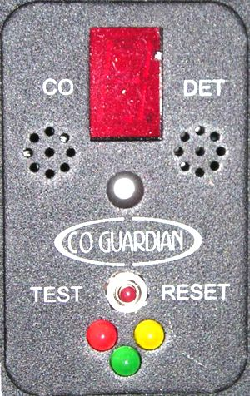
\includegraphics{../Diagrams/co}}


The CO Guardian Aero 252F CO Monitor provides visual and aural indications of CO levels that exceed 40 PPM. The CO Monitor is located on the lower left side of the cockpit, ahead of the fuel selector. It is powered from the Main Bus, and has an ON/OFF toggle switch to its right.

The unit is designed to operate in temperatures of -1\textdegree C to 49\textdegree C.

\textbf{Self-Test} --- The unit performs a self-test upon power application, or when the TEST/RESET button on its face is pressed. A successful self-test provides the following indications in sequence:
\begin{itemize}
\item Display shows 0 
\item Aural alert sounds two beeps 
\item Green, Yellow and Red LEDs flash in sequence 
\item Display counts up from 1 to 9 then 0 
\item Aural alert sounds one beep 
\item Yellow LED flashes 
\item Display goes blank 
\item Green LED remains illuminated, with the Yellow and Red LED OFF 
\end{itemize}
\textbf{Digital Display} --- The digital display remains blank for CO concentrations of less than 40 PPM. It flashes two digits in sequence for CO concentrations of between 40 and 99 PPM (e.g. alternating 5 and 0 indicates 50 PPM). CO concentrations of greater than 100 PPM will be displayed as a single, steady digit equal to the hundreds unit (e.g. steady 5 means 500 PPM). The digital display shows the CO level without delay.

\textbf{Aural Indications} --- The unit has a built-in speaker. It is not connected to the intercom. CO concentrations of greater than 50 for a specified time delay are annunciated by beeps and flashes of the Yellow LED or Red LED.


\textbf{Normal Indications} --- If the CO concentration is less than 40 PPM, the Green light will be illuminated, the display will be blank and there will be no aural alerts. If the CO concentration is between 40 and 50 PPM, the display will alternate between 4 and 0, and the Green light will remain illuminated.

\begin{minipage}{\textwidth}
\textbf{CO Alarm Indications} --- CO values of 50 PPM or greater are indicated as follows:
\begin{center}
\begin{tabular}
{|c|c|c|} \hline CO Conc. (PPM) & Aural Alarm Delay& LED that will be lit\tabularnewline \hline \hline Less than 50 & No alarm& Green\tabularnewline \hline 50-70& 10 minutes & Yellow\tabularnewline \hline 70-150 & 5 minutes& Red\tabularnewline \hline 200& 3 minutes & Red\tabularnewline \hline 300& 1 minute& Red\tabularnewline \hline 400& No delay & Red\tabularnewline \hline 
\end{tabular}
\end{center}
\end{minipage}

\textbf{System Failures} --- System failures are indicated as follows:
\begin{itemize}
\item Flashing Green, Red and Yellow LEDs + beep every 30s CO --- sensor failure 
\item Flashing Red LED + beep every 30s --- temperature sensor failure 
\item Flashing Yellow LED + beep every 30s --- humidity sensor failure 
\item Any other combination of flashing LEDs + beep every 30s --- micro-controller failure 
\end{itemize}

\section{FIRE EXTINGUISHER}

A 2.5 lb halon fire extinguisher is mounted in a bracket on the floor on the left side  of the cockpit below the rear seat throttle. The cockpit must be ventilated after using the fire extinguisher.

\section{EMERGENCY LOCATOR TRANSMITTER} 
\piccaption{ELT Remote Control} 
\parpic[r]{
\includegraphics{../Diagrams/elt1}}

The aircraft is fitted with an ACK E-04 406 MHz Emergency Locater Transmitter (ELT). The ELT is mounted in in the aft baggage area, on a tray at the forward right side. The ELT remote control is located on the upper right side of the instrument panel. The ELT may be selected ON by a momentary press of the ON button on the left side of the remote control. The red ON light will flash when the ELT is transmitting. The ELT may be selected OFF by a momentary press of the RESET button. An aural alert will sound every 50 s when the ELT is transmitting.

The ELT has a three-position switch. This switch should be in the ARMED position for flight, in which case it is covered with a red plastic cap which retains it in the ARMED position. The ON position is used to force the ELT to transmit after removing it from the aircraft and connecting the telescopic antenna. 
\begin{figure}
[htb]

% 
\centering 
\begin{minipage}{3in}

%
\centering 
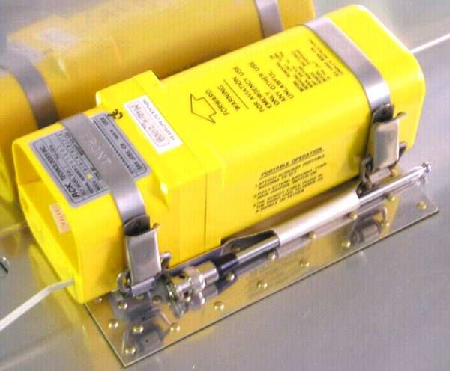
\includegraphics[scale=0.8]{../Diagrams/elt2} \caption{ELT in Tray} 
\end{minipage}

% 
\qquad 
\begin{minipage}{3in}

%
\centering 
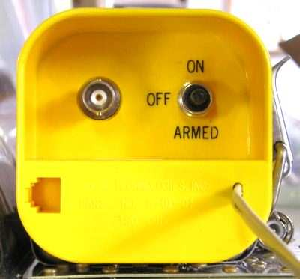
\includegraphics[scale=1]{../Diagrams/elt3} \caption{ELT Main Control}

% 
\end{minipage}

% 
\end{figure}

Following an emergency landing, the ELT may be removed from the aircraft if required. It is secured to the tray by two over-centre locks on band-clamps. The phone line going to the remote transmitter and the antenna coax cable must both be removed. The loose end of the phone line may be clipped into the receptacle on the ELT to make a loop that can be used as a handle. There is a telescopic antenna clipped to the mounting tray which must be connected to the coax mount on the ELT to allow it to transmit once it is removed from the aircraft. 

\section{FIRST AID KIT}
A first aid kit in a red zippered pouch is attached to the left side of the rear cockpit side wall.

\cleardoublepage 
